\documentclass[a4paper]{amsart}
\usepackage{fullpage}
\usepackage{verbatim}
\usepackage{tikz}
\usetikzlibrary{knots,intersections,decorations.pathreplacing,hobby}
\usepackage{xr-hyper}
\usepackage{hyperref}
\setlength{\textheight}{10.4in}
\setlength{\topmargin}{-0.5in}

\externaldocument{../notes/knots_and_surfaces}

\newcommand{\Braid}     {\operatorname{Braid}}

\newcommand{\N}         {\mathbb{N}}
\newcommand{\Z}         {\mathbb{Z}}
\newcommand{\R}         {\mathbb{R}}
\newcommand{\C}         {\mathbb{C}}

\newcommand{\al}        {\alpha}
\newcommand{\bt}        {\beta}
\newcommand{\ep}        {\epsilon}
\newcommand{\tht}       {\theta}

\newcommand{\Sg}        {\Sigma}

\newcommand{\ab}        {\overline{a}}
\newcommand{\bb}        {\overline{b}}
\newcommand{\cb}        {\overline{c}}
\newcommand{\db}        {\overline{d}}
\newcommand{\eb}        {\overline{e}}
\newcommand{\fb}        {\overline{f}}
\newcommand{\gb}        {\overline{g}}
\newcommand{\pb}        {\overline{p}}
\newcommand{\qb}        {\overline{q}}
\newcommand{\rb}        {\overline{r}}
\newcommand{\ub}        {\overline{u}}
\newcommand{\vb}        {\overline{v}}
\newcommand{\wb}        {\overline{w}}
\newcommand{\xb}        {\overline{x}}
\newcommand{\yb}        {\overline{y}}
\newcommand{\zb}        {\overline{z}}

\newcommand{\tu}        {\widetilde{u}}

\newcommand{\lk}        {\operatorname{lk}}
\newcommand{\ip}[1]     {\langle #1\rangle}
\newcommand{\un}[1]     {\langle\!\langle #1\rangle\!\rangle}
\newcommand{\st}        {\;|\;}
\newcommand{\tm}        {\times}
\newcommand{\ov}        {\overline}
\newcommand{\sse}       {\subseteq}
\newcommand{\sm}        {\setminus}

\renewcommand{\:}       {\colon}


\tikzset{every path/.style={blue,ultra thick}, every node/.style={transform shape, knot crossing, inner sep=2.5pt}}

\def\SOLS{1}
\newcommand{\mk}{}
\newcommand{\mks}[1]{}

\makeatletter

% An environment for a solution that is included inline.
\newenvironment{SolutionInline}{{\noindent \bf Solution:}}{}

% An environment that makes a solution completely invisible.
\newenvironment{SolutionHidden}
 {\@bsphack
  \let\do\@makeother\dospecials\catcode`\^^M\active
  \def\verbatim@processline{}%
 \verbatim@start}%
{\@esphack\par\vspace{2ex}}

%\newenvironment{solution}{\SolutionInline}{\endSolutionInline}

\ifx\SOLS\undefined
\newcommand{\soltitle}{}
\newenvironment{rubric}{}{}
\newenvironment{solution}{\SolutionHidden}{\endSolutionHidden}
\else
\newcommand{\soltitle}{ --- Solutions}
\newenvironment{rubric}{\SolutionHidden}{\endSolutionHidden}
\newenvironment{solution}{\SolutionInline}{\endSolutionInline}
\fi

\makeatother

\theoremstyle{definition}
\newtheorem{exercise}{Exercise}
%\numberwithin{exercise}{section}



\newtheorem*{proposition*}{Proposition}

\title{Knots and Surfaces Problems}

\begin{document}

\tikzset{every path/.style={blue,very thick}, every node/.style={transform shape, knot crossing, inner sep=2.5pt}}

\maketitle

\begin{exercise}
 Show, using a piece of string, that the following two pictures represent the same knot:
 \begin{center}
  \begin{tikzpicture}
   \begin{scope}
    \node (a) at ( 0.00, 1.00) {};
    \node (b) at ( 0.00, 0.00) {};
    \node (c) at ( 0.00,-1.00) {};
    \draw (a.center) 
     .. controls (a.4 south east) and (b.4 north east) .. (b) 
     .. controls (b.4 south west) and (c.4 north west) .. (c.center) 
     .. controls (c.8 south east) and (a.8 north east) .. (a)
     .. controls (a.4 south west) and (b.4 north west) .. (b.center)
     .. controls (b.4 south east) and (c.4 north east) .. (c)
     .. controls (c.8 south west) and (a.8 north west) .. (a.center);
   \end{scope}
   \begin{scope}[xshift=4cm,yshift=0cm,scale=0.5]
    \begin{scope}[rotate=  0] \node (a) at (0,-1) {}; \end{scope}
    \begin{scope}[rotate=120] \node (b) at (0,-1) {}; \end{scope}
    \begin{scope}[rotate=240] \node (c) at (0,-1) {}; \end{scope}
    \draw (a) .. controls (a.4 north west) and (c.4 north east) .. (c.center);
    \draw (b) .. controls (b.4 north west) and (a.4 north east) .. (a.center);
    \draw (c) .. controls (c.4 north west) and (b.4 north east) .. (b.center);
    \draw (a.center) .. controls (a.16 south west) and (c.16 south east) .. (c);
    \draw (b.center) .. controls (b.16 south west) and (a.16 south east) .. (a);
    \draw (c.center) .. controls (c.16 south west) and (b.16 south east) .. (b);
   \end{scope}
  \end{tikzpicture}
 \end{center}
\end{exercise}
\begin{solution}
 See the video on the course web page (\url{http://goo.gl/cU443p}).
\end{solution}

\begin{exercise}
 There are only five link diagrams with one component and at most one crossing:
 \begin{center}
  \begin{tikzpicture}[scale=0.9]
   \begin{scope}
    \draw (0,0) circle(1);
   \end{scope}
   \begin{scope}[xshift=3cm]
    \node (a) at (0,0) {};
    \draw (a) .. controls (a.16 north east) and (a.16 north west) ..
          (a.center) .. controls (a.16 south east) and (a.16 south west) .. (a);
   \end{scope}
   \begin{scope}[xshift=6cm]
    \node (a) at (0,0) {};
    \draw (a.center) .. controls (a.16 north east) and (a.16 north west) ..
          (a) .. controls (a.16 south east) and (a.16 south west) .. (a.center);
   \end{scope}
   \begin{scope}[xshift=12cm]
    \node (a) at ( 1,0) {};
    \node (b) at (-1,0) {};
    \draw (a) .. controls (a.8 north east) and (b.8 north) ..
          (b.center) .. controls (b.8 south) and (a.8 south east) .. 
          (a.center) .. controls (a.8 north west) and (a.8 south west) .. (a);
   \end{scope}
   \begin{scope}[xshift=9cm]
    \node (a) at ( 1,0) {};
    \node (b) at (-1,0) {};
    \draw (a.center) .. controls (a.8 north east) and (b.8 north) ..
          (b.center) .. controls (b.8 south) and (a.8 south east) .. 
          (a) .. controls (a.8 north west) and (a.8 south west) .. (a.center);
   \end{scope}
  \end{tikzpicture}
 \end{center}
 They are all R-equivalent, so they all represent the unknot.  Now
 consider link diagrams with precisely two crossings.  There are a
 large number of diagrams which can be divided into two separate
 pieces with no crossings in common.  A few of these are shown below:
 \begin{center}
  \begin{tikzpicture}[scale=0.5]
   \begin{scope}
    \draw[red] (0,0) circle(2);  
    \node (a) at (0,0) {};
    \draw (a) .. controls (a.16 north east) and (a.16 north west) ..
          (a.center) .. controls (a.16 south east) and (a.16 south west) .. (a);
   \end{scope}
   \draw[dotted,black] (4,-2) -- (4,2);
   \begin{scope}[xshift=8cm,scale=2]
    \node (a) at ( 1,0) {};
    \node (b) at (-1,0) {};
    \draw[red] (a) .. controls (a.8 north east) and (b.8 north) ..
          (b.center) .. controls (b.8 south) and (a.8 south east) .. 
          (a.center) .. controls (a.8 north west) and (a.8 south west) .. (a);
    \begin{scope}[xshift=-0.4cm,scale=0.3]
     \node (a) at ( 1,0) {};
     \node (b) at (-1,0) {};
     \draw (a) .. controls (a.8 north east) and (b.8 north) ..
           (b.center) .. controls (b.8 south) and (a.8 south east) .. 
           (a.center) .. controls (a.8 north west) and (a.8 south west) .. (a);
    \end{scope}
   \end{scope}
   \begin{scope}[xshift=14cm]
    \begin{scope}
     \node (a) at (0,0) {};
     \draw[red] (a) .. controls (a.16 north east) and (a.16 north west) ..
           (a.center) .. controls (a.16 south east) and (a.16 south west) .. (a);
    \end{scope}
    \begin{scope}[xshift=2cm]
     \node (a) at (0,0) {};
     \draw (a.center) .. controls (a.16 north east) and (a.16 north west) ..
           (a) .. controls (a.16 south east) and (a.16 south west) .. (a.center);
    \end{scope}   
   \end{scope}
   \draw[dotted,black] (12,-2) -- (12,2);
  \end{tikzpicture}
 \end{center}
 Draw all possible link diagrams that \textbf{cannot} be split in this
 uninteresting way.  How many different knots or links do these
 represent? 
\end{exercise}
\begin{solution}
 This is surprisingly hard to get right.  There are six possible link universes,
 as follows: 
 \begin{center}
  \begin{tikzpicture}[scale=0.6]
   \begin{scope}
    \draw(-3,2) node[anchor=north west] {\Large $1$};
    \draw[thin,black] (-3,-2) rectangle (3,2);
    \draw (-2,-1) -- (2,-1) -- (0.5, 0.5) -- (-0.5, 0.5) -- (-2,-1);
    \draw (-2, 1) -- (2, 1) -- (0.5,-0.5) -- (-0.5,-0.5) -- (-2, 1);
   \end{scope}
   \begin{scope}[xshift=6cm]
    \draw(-3,2) node[anchor=north west] {\Large $2$};
    \draw[thin,black] (-3,-2) rectangle (3,2);
    \draw (-2,-1) -- (2,-1) -- (0.5, 0.5) -- (-0.5, 0.5) -- (-1.5,-0.5) --
          (-1.5,0.5) -- (-0.5,-0.5) -- (0.5,-0.5) -- (2,1) -- (-2,1) -- (-2,-1);
   \end{scope}
   \begin{scope}[xshift=12cm]
    \draw(-3,2) node[anchor=north west] {\Large $3$};
    \draw[thin,black] (-3,-2) rectangle (3,2);
    \draw (-2,-1) -- (2,-1) -- (0.5, 0.5) -- (-1.5, 0.5) -- (-0.7,-0.3) --
          (-0.7,0.3) -- (-1.5,-0.5) -- (0.5,-0.5) -- (2,1) -- (-2,1) -- (-2,-1);
   \end{scope}
   \begin{scope}[yshift=-4cm]
    \draw(-3,2) node[anchor=north west] {\Large $4$};
    \draw[thin,black] (-3,-2) rectangle (3,2);
    \draw (-2,-1) -- (2,-1) -- (0.5,0.5) -- (0.5,-0.5) -- (2,1) --
          (-2,1) -- (-0.5,-0.5) -- (-0.5,0.5) -- (-2,-1);
   \end{scope}
   \begin{scope}[xshift=6cm,yshift=-4cm]
    \draw(-3,2) node[anchor=north west] {\Large $5$};
    \draw[thin,black] (-3,-2) rectangle (3,2);
    \draw (-2,-1) -- (0.5,-1) -- (2,0.5) -- (2,-0.5) -- (0.5,1) -- 
          (-2,1) -- (-0.5,-0.5) -- (-0.5,0.5) -- (-2,-1);
   \end{scope}
   \begin{scope}[xshift=12cm,yshift=-4cm]
    \draw(-3,2) node[anchor=north west] {\Large $6$};
    \draw[thin,black] (-3,-2) rectangle (3,2);
    \draw (-0.5,-1) -- (0.5,-1) -- (2,0.5) -- (2,-0.5) -- (0.5,1) -- 
          (-0.5,1) -- (-2,-0.5) -- (-2,0.5) -- (-0.5,-1);
   \end{scope}
  \end{tikzpicture}
 \end{center}
 To see this, note that the arcs can either join a crossing to itself,
 or they can bridge between the two crossings.  If there are no
 bridges, then the universe disconnects into two pieces, and we were
 told to ignore that case.  There cannot be an odd number of bridges,
 because it would then be impossible to match up the remaining loose
 ends to make loops.  If there are four bridges, then the only
 possibility is picture 1.  If there are two bridges, then there must
 also be two loops.  The loops might both be small (pictures 4,5 and
 6), or one of them they might wrap all the way around the outside
 (pictures 2 and 3).  Both of the loops might be nestled in
 between the pair of bridges, as in picture 4.  Alternatively, one
 might be between the bridges, and the other might be outside
 (pictures 3 and 5) or both might be outside (pictures 2 and 6).  We
 can get additional pictures by rotating pictures 2, 3 and 5 through
 180 degrees, but that rotation is an ambient isotopy, so we regard
 the rotated diagram as being equivalent to the original one.

 Each of pictures 2 to 6 has a small triangle.  If we choose
 overcrossings and undercrossings to make the universe into a link
 diagram, we can immediately remove the small triangle by a
 Reidemeister move of type 1.  This will leave a diagram with only one
 crossing, which can again be removed by a Reidemeister move of type
 1, leaving the unknot.  On the other hand, there are four possible
 ways to specify the crossings in picture 1, each of which gives two
 component circles.  Two of the four possibilities give a pair of
 unlinked circles; the other two give a Hopf link.  Thus, there are
 three possible outcomes altogether: the unknot, the unlink and the
 Hopf link.
\end{solution}

\begin{exercise}
 Show that the following pairs of link diagrams are $R$-equivalent.
 \begin{center}
  \begin{tikzpicture}[scale=0.5]
   \begin{scope}
    \node (p) at (-5, 0) {};
    \node (q) at ( 5, 0) {};
    \node (a) at (-2, 1) {};
    \node (b) at ( 0, 1) {};
    \node (c) at ( 2, 1) {};
    \node (d) at (-2,-1) {};
    \node (e) at ( 0,-1) {};
    \node (f) at ( 2,-1) {};
    \draw 
     (a)        .. controls (a.8 south east) and (b.8 south west) ..
     (b.center) .. controls (b.8 north east) and (c.8 north west) ..
     (c)        .. controls (c.8 south east) and (f.8 north east) ..
     (f)        .. controls (f.8 south west) and (e.8 south east) ..
     (e.center) .. controls (e.8 north west) and (d.8 north east) ..
     (d)        .. controls (d.8 south west) and (p.16 south) ..
     (p.center) .. controls (p.16 north) and (a.8 north west) ..
     (a);
    \draw 
     (c.center) .. controls (c.8 south west) and (b.8 south east) ..
     (b)        .. controls (b.8 north west) and (a.8 north east) ..
     (a.center) .. controls (a.8 south west) and (d.8 north west) ..
     (d.center) .. controls (d.8 south east) and (e.8 south west) ..
     (e)        .. controls (e.8 north east) and (f.8 north west) ..
     (f.center) .. controls (f.8 south east) and (q.16 south) ..
     (q.center) .. controls (q.16 north) and (c.8 north east) ..
     (c.center);
    \draw (-3.6,0) circle(0.7);
    \draw ( 3.6,0) circle(0.7);
   \end{scope}
   \draw[black] (7,0) node{\Huge and };
   \begin{scope}[xshift=10cm,draw=red]
    \draw[red] (0.0,0) circle(1);
    \draw[red] (2.4,0) circle(1);
    \draw[red] (4.8,0) circle(1);
    \draw[red] (7.2,0) circle(1);
   \end{scope}
  \end{tikzpicture}
 \end{center}
 \begin{center}
  \begin{tikzpicture}[scale=0.5]
   \begin{scope}
    \node (a) at ( 0.00, 1.00) {};
    \node (b) at ( 0.00,-1.00) {};
    \draw (a.center) .. controls (a.4 south east) and (b.4 north east) ..
          (b) .. controls (b.16 south west) and (a.16 north west) .. (a.center);
    \draw (a) .. controls (a.4 south west) and (b.4 north west) ..
          (b.center) .. controls (b.16 south east) and (a.16 north east) .. (a);
   \end{scope}
   \draw[black] (3,0) node{\Huge and };
   \begin{scope}[xshift=6cm]
    \node (a) at ( 0.00, 1.00) {};
    \node (b) at ( 0.00,-1.00) {};
    \draw[red] (a) .. controls (a.4 south east) and (b.4 north east) ..
          (b.center) .. controls (b.16 south west) and (a.16 north west) .. (a);
    \draw[red] (a.center) .. controls (a.4 south west) and (b.4 north west) ..
          (b) .. controls (b.16 south east) and (a.16 north east) .. (a.center);
   \end{scope}
  \end{tikzpicture}
 \end{center}
\end{exercise}
\begin{solution}
 For the first pair of diagrams, we can use the following sequence of moves:
 \begin{center}
  \begin{tikzpicture}[scale=0.35]
   \begin{scope}
    \node (p) at (-5, 0) {};
    \node (q) at ( 5, 0) {};
    \node (a) at (-2, 1) {};
    \node (b) at ( 0, 1) {};
    \node (c) at ( 2, 1) {};
    \node (d) at (-2,-1) {};
    \node (e) at ( 0,-1) {};
    \node (f) at ( 2,-1) {};
    \draw 
     (a)        .. controls (a.8 south east) and (b.8 south west) ..
     (b.center) .. controls (b.8 north east) and (c.8 north west) ..
     (c)        .. controls (c.8 south east) and (f.8 north east) ..
     (f)        .. controls (f.8 south west) and (e.8 south east) ..
     (e.center) .. controls (e.8 north west) and (d.8 north east) ..
     (d)        .. controls (d.8 south west) and (p.16 south) ..
     (p.center) .. controls (p.16 north) and (a.8 north west) ..
     (a);
    \draw 
     (c.center) .. controls (c.8 south west) and (b.8 south east) ..
     (b)        .. controls (b.8 north west) and (a.8 north east) ..
     (a.center) .. controls (a.8 south west) and (d.8 north west) ..
     (d.center) .. controls (d.8 south east) and (e.8 south west) ..
     (e)        .. controls (e.8 north east) and (f.8 north west) ..
     (f.center) .. controls (f.8 south east) and (q.16 south) ..
     (q.center) .. controls (q.16 north) and (c.8 north east) ..
     (c.center);
    \draw (-3.6,0) circle(0.7);
    \draw ( 3.6,0) circle(0.7);
    \draw[thin,black] (-7,-3) rectangle (7,3);
   \end{scope}
   \begin{scope}[xshift=14cm]
    \node (p) at (-5, 0) {};
    \node (q) at ( 5, 0) {};
    \node (a) at (-2, 1) {};
    \node (b) at ( 0, 1) {};
    \node (c) at ( 2, 1) {};
    \node (d) at (-2,-1) {};
    \node (e) at ( 0,-1) {};
    \node (f) at ( 2,-1) {};
    \draw 
     (a)        .. controls (a.8 south east) and (b.8 south west) ..
     (b.center) .. controls (b.8 north east) and (c.8 north west) ..
     (c)        .. controls (c.8 south east) and (f.8 north east) ..
     (f)        .. controls (f.8 south west) and (e.8 south east) ..
     (e.center) .. controls (e.8 north west) and (d.8 north east) ..
     (d)        .. controls (d.8 south west) and (p.16 south) ..
     (p.center) .. controls (p.16 north) and (a.8 north west) ..
     (a);
    \draw 
     (c.center) .. controls (c.8 south west) and (b.8 south east) ..
     (b)        .. controls (b.8 north west) and (a.8 north east) ..
     (a.center) .. controls (a.8 south west) and (d.8 north west) ..
     (d.center) .. controls (d.8 south east) and (e.8 south west) ..
     (e)        .. controls (e.8 north east) and (f.8 north west) ..
     (f.center) .. controls (f.8 south east) and (q.16 south) ..
     (q.center) .. controls (q.16 north) and (c.8 north east) ..
     (c.center);
    \draw[draw=white,double=blue ,ultra thick,double distance=1.2pt] (-5,0) circle(0.7);
    \draw[draw=white,double=blue ,ultra thick,double distance=1.2pt] ( 5,0) circle(0.7);
    \draw[thin,black] (-7,-3) rectangle (7,3);
   \end{scope}
   \begin{scope}[xshift=28cm]
    \node (p) at (-3.5, 0) {};
    \node (q) at ( 3.5, 0) {};
    \node (a) at (-2, 1) {};
    \node (b) at ( 0, 1) {};
    \node (c) at ( 2, 1) {};
    \node (d) at (-2,-1) {};
    \node (e) at ( 0,-1) {};
    \node (f) at ( 2,-1) {};
    \draw 
     (a)        .. controls (a.8 south east) and (b.8 south west) ..
     (b.center) .. controls (b.8 north east) and (c.8 north west) ..
     (c)        .. controls (c.8 south east) and (f.8 north east) ..
     (f)        .. controls (f.8 south west) and (e.8 south east) ..
     (e.center) .. controls (e.8 north west) and (d.8 north east) ..
     (d)        .. controls (d.8 south west) and (p.16 south) ..
     (p.center) .. controls (p.16 north) and (a.8 north west) ..
     (a);
    \draw 
     (c.center) .. controls (c.8 south west) and (b.8 south east) ..
     (b)        .. controls (b.8 north west) and (a.8 north east) ..
     (a.center) .. controls (a.8 south west) and (d.8 north west) ..
     (d.center) .. controls (d.8 south east) and (e.8 south west) ..
     (e)        .. controls (e.8 north east) and (f.8 north west) ..
     (f.center) .. controls (f.8 south east) and (q.16 south) ..
     (q.center) .. controls (q.16 north) and (c.8 north east) ..
     (c.center);
    \draw (-5,0) circle(0.7);
    \draw ( 5,0) circle(0.7);
    \draw[thin,black] (-7,-3) rectangle (7,3);
   \end{scope}
   \begin{scope}[yshift=-6cm]
    \node (p) at (-3.5, 0) {};
    \node (q) at ( 3.5, 0) {};
    \node (a) at (-2, 1) {};
    \node (b) at ( 0, 1) {};
    \node (c) at ( 2, 1) {};
    \node (d) at (-2,-1) {};
    \node (e) at ( 0,-1) {};
    \node (f) at ( 2,-1) {};
    \draw 
     (b.center) .. controls (b.8 north east) and (c.8 north west) ..
     (c.center) .. controls (c.8 south east) and (f.8 north east) ..
     (f.center) .. controls (f.8 south west) and (e.8 south east) ..
     (e.center) .. controls (e.8 north west) and (d.8 north east) ..
     (d)        .. controls (d.8 south west) and (p.16 south) ..
     (p.center) .. controls (p.16 north) and (a.8 north west) ..
     (a)        .. controls (a.8 south east) and (b.8 south west) ..
     (b.center);
    \draw 
     (b)        .. controls (b.8 north west) and (a.8 north east) ..
     (a.center) .. controls (a.8 south west) and (d.8 north west) ..
     (d.center) .. controls (d.8 south east) and (e.8 south west) ..
     (e)        .. controls (e.8 north east) and (f.8 north west) ..
     (b);
    \draw (-5,0) circle(0.7);
    \draw ( 5,0) circle(0.7);
    \draw[thin,black] (-7,-3) rectangle (7,3);
   \end{scope}
   \begin{scope}[yshift=-6cm,xshift=14cm]
    \node (p) at (-3.5, 0) {};
    \node (q) at ( 3.5, 0) {};
    \node (a) at (-2, 1) {};
    \node (b) at ( 0, 1) {};
    \node (c) at ( 2, 1) {};
    \node (d) at (-2,-1) {};
    \node (e) at ( 0,-1) {};
    \node (f) at ( 2,-1) {};
    \draw 
     (b.center) .. controls (b.8 north east) and (c.8 north west) ..
     (c.center) .. controls (c.8 south east) and (f.8 north east) ..
     (f.center) .. controls (f.8 south west) and (e.8 south east) ..
     (e.center) .. controls (e.8 north west) and (d.8 north east) ..
     (b.center);
    \draw 
     (b)        .. controls (b.8 north west) and (a.8 north east) ..
     (a.center) .. controls (a.8 south west) and (d.8 north west) ..
     (d.center) .. controls (d.8 south east) and (e.8 south west) ..
     (e)        .. controls (e.8 north east) and (f.8 north west) ..
     (b);
    \draw (-4.5,0) circle(0.7);
    \draw ( 4.5,0) circle(0.7);
    \draw[thin,black] (-7,-3) rectangle (7,3);
   \end{scope}
   \begin{scope}[yshift=-6cm,xshift=28cm]
    \draw[thin,black] (-7,-3) rectangle (7,3);
    \draw (-4.5,0) circle(0.8);
    \draw (-1.5,0) circle(0.8);
    \draw ( 1.5,0) circle(0.8);
    \draw ( 4.5,0) circle(0.8);
   \end{scope}
  \end{tikzpicture}
 \end{center}
 All the Reidemeister moves here are of type 2.  In the first and
 second steps we have performed two Reidemeister moves at the same
 time, but the remaining three steps just consist of a single
 Reidemeister move.


 For the second pair of diagrams, we use a Reidemeister move of
 type 1, then a move of type 3, then another move of type 1.
 \begin{center}
  \begin{tikzpicture}[scale=0.5]
   \draw[thin,black] (-2,-2) rectangle (25.5,2);
   \draw[thin,black] (2.7,2) -- (2.7,-2);
   \draw[thin,black] ( 8.6,2) -- ( 8.6,-2);
   \draw[thin,black] (14.6,2) -- (14.6,-2);
   \draw[thin,black] (20.6,2) -- (20.6,-2);
   \begin{scope}
    \draw[rounded corners] (-1,0) -- (-1,1) -- (1,1) -- (1,-0.4);
    \draw[rounded corners] (1,-0.8) -- (1,-1) -- (-1,-1) -- (-1,0);
    \draw[red,rounded corners] (0.5,0) -- (0.5,-0.6) -- (2,-0.6) -- (2,0.6) -- (1.2,0.6);
    \draw[red,rounded corners] (0.8,0.6) -- (0.5,0.6) -- (0.5,0); 
   \end{scope}
   \begin{scope}[xshift=4.5cm]
    \draw[rounded corners] (-1,0) -- (-1,1) -- (1,1) -- (1,-0.4);
    \draw[rounded corners] (1,-0.8) -- (1,-1) -- (-1,-1) -- (-1,0);
    \draw[red,rounded corners]
      (0.5,0) -- (0.5,-0.6) -- (1.4,-0.6) -- (2.6,0.6) -- (3.4,0.6) --
      (3.4,-0.6) -- (2.6,-0.6) -- (2.1,-0.1);
    \draw[red,rounded corners]
      (1.9, 0.1) -- (1.4,0.6) -- (1.2,0.6);
    \draw[red,rounded corners] (0.8,0.6) -- (0.5,0.6) -- (0.5,0); 
   \end{scope}
   \begin{scope}[xshift=10.5cm]
    \draw[rounded corners] (-1,0) -- (-1,1) -- (3,1) -- (3,0.8);
    \draw[rounded corners] (3,0.4) -- (3,-1) -- (-1,-1) -- (-1,0);
    \draw[red,rounded corners]
     (0.5,0) -- (0.5,-0.6) -- (1.3,-0.6) -- (2.6,0.6) -- (3.4,0.6) --
     (3.4,-0.6) -- (3.2,-0.6);
    \draw[red,rounded corners]
     (2.8,-0.6) -- (2.6,-0.6) -- (2.1,-0.1);
    \draw[red,rounded corners]
     (1.9,0.1) -- (1.3,0.6) -- (0.5,0.6) -- (0.5,0); 
   \end{scope}
   \begin{scope}[xshift=16.5cm]
    \draw[rounded corners] (-1,0) -- (-1,1) -- (3,1) -- (3,0.8);
    \draw[rounded corners] (3,0.4) -- (3,-1) -- (-1,-1) -- (-1,0);
    \draw[red,rounded corners]
     (0.5,0) -- (0.5,-0.6) -- (2.8,-0.6);
    \draw[red,rounded corners]
     (3.2,-0.6) -- (3.4,-0.6) -- (3.4,0.6) -- (0.5,0.6) -- (0.5,0); 
   \end{scope}
   \begin{scope}[xshift=22.5cm]
    \draw[rounded corners] (-1,0) -- (-1,1) -- (1,1) -- (1,0.8);
    \draw[rounded corners] (1,0.4) -- (1,-1) -- (-1,-1) -- (-1,0);
    \draw[red,rounded corners]
     (0.5,0) -- (0.5,-0.6) -- (0.8,-0.6);
    \draw[red,rounded corners]
     (1.2,-0.6) -- (2,-0.6) -- (2,0.6) -- (0.5,0.6) -- (0.5,0); 
   \end{scope}
  \end{tikzpicture}
 \end{center}
\end{solution}

\begin{exercise}
 Show that given any knot universe you can choose the crossings so
 that the resulting knot diagram represents the unknot.  (This will
 probably take some experimentation.  If you fail to do it with pen
 and paper, I highly recommend getting a piece of string and trying to
 do it with that.)  Can you prove that your method always gives the
 unknot?
\end{exercise}
\begin{solution}
 Start with a knot universe, so none of the crossings are marked as
 undercrossings or overcrossings.  Choose a point $a$ on one of the
 arcs, and start walking around from there.  Each time you get to a
 crossing that has not already been marked, mark it so that your
 current strand is the upper one.  Eventually you will get back to
 $a$, and all the crossings will be marked.  For example, consider the
 following picture:
 \begin{center}
  \begin{tikzpicture}
   \begin{scope}
    \begin{scope}
     \node (a) at (-1.0, 1) {};
     \node (b) at (-2, 0) {};
     \node (c) at (-1.0,-1) {};
     \node (d) at ( 1.0, 1) {};
     \node (e) at ( 2, 0) {};
     \node (f) at ( 1.0,-1) {};
     \draw (a.center) .. controls (-0.5,1.4) and (0.5,1.4) ..
           (d.center) .. controls (d.8 south east) and (e.8 north west) ..
           (e.center) .. controls (e.8 south east) and (f.8 south) ..
           (f.center) .. controls (f.8 north) and (d.8 south) ..
           (d.center) .. controls (d.8 north) and (e.8 north east) ..
           (e.center) .. controls (e.8 south west) and (f.8 north east) ..
           (f.center) .. controls (0.5,-1.4) and (-0.5,-1.4) ..
           (c.center) .. controls (c.8 north west) and (b.8 south east) ..
           (b.center) .. controls (b.8 north west) and (a.8 north) ..
           (a.center) .. controls (a.8 south) and (c.8 north) ..
           (c.center) .. controls (c.8 south) and (b.8 south west) ..
           (b.center) .. controls (b.8 north east) and (a.8 south west) ..
           (a.center) ;
     \draw[black] (d) node[anchor=west] {$1$};
     \draw[black] (e) node[anchor=west] {$2$};
     \draw[black] (f) node[anchor=west] {$3$};
     \draw[black] (c) node[anchor=east] {$4$};
     \draw[black] (b) node[anchor=east] {$5$};
     \draw[black] (a) node[anchor=east] {$6$};
     \draw[->] (0,1.3) -- +(0.01,0);
    \end{scope}
   \end{scope}
   \begin{scope}[xshift=7cm]
    \begin{scope}
     \node (a) at (-1.0, 1) {};
     \node (b) at (-2, 0) {};
     \node (c) at (-1.0,-1) {};
     \node (d) at ( 1.0, 1) {};
     \node (e) at ( 2, 0) {};
     \node (f) at ( 1.0,-1) {};
     \draw (a)        .. controls (-0.5,1.4) and (0.5,1.4) ..
           (d.center) .. controls (d.8 south east) and (e.8 north west) ..
           (e.center) .. controls (e.8 south east) and (f.8 south) ..
           (f.center) .. controls (f.8 north) and (d.8 south) ..
           (d)        .. controls (d.8 north) and (e.8 north east) ..
           (e)        .. controls (e.8 south west) and (f.8 north east) ..
           (f)        .. controls (0.5,-1.4) and (-0.5,-1.4) ..
           (c.center) .. controls (c.8 north west) and (b.8 south east) ..
           (b.center) .. controls (b.8 north west) and (a.8 north) ..
           (a.center) .. controls (a.8 south) and (c.8 north) ..
           (c)        .. controls (c.8 south) and (b.8 south west) ..
           (b)        .. controls (b.8 north east) and (a.8 south west) ..
           (a);
    \end{scope}
   \end{scope}
  \end{tikzpicture}
 \end{center}
 Starting from the position marked with an arrow, we visit crossings
 1, 2 and 3, and we mark them as overcrossings.  We then revisit
 crossings 1, 2 and 3, this time passing underneath.  We then cross
 over to the left hand part of the picture, and visit crossings 4, 5
 and 6, marking them as overcrossings.  We then revisit crossings 4, 5
 and 6, passing underneath.  This brings us back to the start.

 The above procedure gives a diagram which corresponds to the unknot.
 To see why, imagine the knot lying close to the $xy$ plane, and just
 bending up or down a little bit at the crossings.  Imagine an
 unknotted circle $C$ lying in the plane $z=1$.  Stretch and pull a
 short section of string near $a$ to move $a$ onto $C$.  Then work
 around the knot, pulling the string up to $C$.  The first time we get
 to each crossing, we will be on top, so there is nothing to stop us
 from moving the string.  The second time we get to each crossing we
 will be on the bottom strand, but the top strand will already have
 been removed, so there will again be nothing in the way.

 There is a video to illustrate this argument at \url{http://goo.gl/cU443p}.
\end{solution}

\begin{exercise}
 Have a look at some of the websites listed on the course webpage.
 Have a read of the wikipedia webpage on knot theory.  How many
 different knots can you draw using diagrams with at most 10
 crossings?  Where can you find pictures of all of them?
\end{exercise}
\begin{solution}
 A table of knots with up to 10 crossings (originally due to Rolfsen)
 can be found here: 
 \begin{center}
  \url{http://katlas.math.toronto.edu/wiki/The\_Rolfsen\_Knot\_Table}
 \end{center}
 Note, however, that this table only includes \emph{prime} knots.
 Many knots can be obtained by splicing together two nontrivial knots,
 like this:
 \begin{center}
  \begin{tikzpicture}
   \fill[lightgray,rounded corners] (-3,-1) rectangle (-1,1);
   \fill[lightgray,rounded corners] ( 3,-1) rectangle ( 1,1);
   \draw (-1, 0.3) -- (1, 0.3);
   \draw (-1,-0.3) -- (1,-0.3);
   \draw[->] (-1, 0.3) -- (0, 0.3);
   \draw[->] ( 1,-0.3) -- (0,-0.3);
  \end{tikzpicture}
 \end{center}
 Knots of this form are considered \emph{composite}, and they are not
 listed in the Rolfsen table.  Any knot can be decomposed into prime
 knots, so this is no great loss.  Moreover, many prime knots are
 different from their mirror images, and only one of each mirror pair
 appears in the Rolfsen table, so this is another source of extra
 knots.  The number of knots in the table can be tabulated as follows:
 \[ \begin{array}{|c|c|c|c|c|c|c|c|c|c|c|c|} \hline
     \text{crossings} & 0 & 1 & 2 & 3 & 4 & 5 & 6 & 7 & 8 & 9 & 10 \\ \hline
     \text{knots}     & 1 & 0 & 0 & 1 & 1 & 2 & 3 & 7 & 21 & 49 & 165
     \\ \hline
    \end{array}
 \]
\end{solution}

\begin{exercise}
 For each of the following link diagrams, find the number of
 components, and mark the crossings positive or negative. 
 \vspace{-4ex}
 \begin{center}
  \begin{tikzpicture}[scale=0.5]
   \begin{scope}
    \node (a) at (0,1) {};
    \node (b) at (2,1) {};
    \node (c) at (3,1) {};
    \node (d) at (1,0) {};
    \node (e) at (2,0) {};
    \node (f) at (3,0) {};
    \draw 
     (b)        .. controls (b.4 north east) and (c.4 north west) ..
     (c.center) .. controls (c.4 south) and (f.4 north) ..
     (f.center) .. controls (f.4 south west) and (e.4 south east) ..
     (e)        .. controls (e.4 north) and (b.4 south) ..
     (b);
    \draw 
     (a)        .. controls (a.8 north east) and (b.8 west) ..
     (b.center) .. controls (b.8 east) and (c.8 west) ..
     (c)        .. controls (c.8 east) .. (3.2,1);
    \draw[rounded corners]
     (3.2,1) -- (4,1) -- (4,3) -- (-1,3) -- (-1,1) -- (-0.8,1);
    \draw
     (-0.8,1) .. controls (-0.1,1) and (a.8 west) ..
     (a.center) .. controls (a.8 east) and (d.8 north) ..
     (d)        .. controls (d.2 south) .. (1,-0.2);
    \draw[rounded corners]
     (1,-0.2) -- (1,-0.5) -- (-1.5,-0.5) -- (-1.5,3.5) -- (4.5,3.5) -- (4.5,0) -- (3.5,0);
    \draw 
     (3.5,0) .. controls (f.4 east) .. 
     (f) .. controls (e.4 east) ..
     (e.center) .. controls (d.4 east) ..
     (d.center) .. controls (d.4 west) and (a.4 south) .. (a);
    \draw[->] (1.5,3.5) -- (1.51,3.5);
    \draw[->] (3.0,0.5) -- (3.0,0.49);
   \end{scope}
   \begin{scope}[xshift=10cm,yshift=1cm]
    \begin{scope}[rotate=  0] \node (a0) at (0,1) {}; \end{scope}
    \begin{scope}[rotate=120] \node (a1) at (0,1) {}; \end{scope}
    \begin{scope}[rotate=240] \node (a2) at (0,1) {}; \end{scope}
    \begin{scope}[rotate= 60] \node (b0) at (0,2) {}; \end{scope}
    \begin{scope}[rotate=180] \node (b1) at (0,2) {}; \end{scope}
    \begin{scope}[rotate=300] \node (b2) at (0,2) {}; \end{scope}
    \draw[blue]
          (b0)        .. controls (b0.4 south west) and (a1.4 north east) ..
          (a1.center) .. controls (a1.4 south west) and (a2.4 south east) ..
          (a2)        .. controls (a2.4 north west) and (b2.4 south east) ..
          (b2.center) .. controls (b2.16 north west) and (b0.16 north east) .. (b0);
    \draw[red]
          (b1)        .. controls (b1.4 south west) and (a2.4 north east) ..
          (a2.center) .. controls (a2.4 south west) and (a0.4 south east) ..
          (a0)        .. controls (a0.4 north west) and (b0.4 south east) ..
          (b0.center) .. controls (b0.16 north west) and (b1.16 north east) .. (b1);
    \draw[green]
          (b2)        .. controls (b2.4 south west) and (a0.4 north east) ..
          (a0.center) .. controls (a0.4 south west) and (a1.4 south east) ..
          (a1)        .. controls (a1.4 north west) and (b1.4 south east) ..
          (b1.center) .. controls (b1.16 north west) and (b2.16 north east) .. (b2);
    \draw[blue ,->] ( 90:2.7) -- +(180:0.1); 
    \draw[red  ,->] (210:2.7) -- +(300:0.1); 
    \draw[green,->] (330:2.7) -- +(420:0.1); 
   \end{scope}
   \begin{scope}[xshift=16cm,yshift=1.5cm,scale=1.5]
    \node (a) at ( 0.00, 1.00) {};
    \node (b) at ( 0.00,-1.00) {};
    \draw[blue] (a.center) .. controls (a.4 south east) and (b.4 north east) ..
                (b) .. controls (b.16 south west) and (a.16 north west) .. (a.center);
    \draw[red]  (a) .. controls (a.4 south west) and (b.4 north west) ..
                (b.center) .. controls (b.16 south east) and (a.16 north east) .. (a);
    \draw[red ,->] (-0.31,0) -- (-0.31, 0.01);
    \draw[blue,->] ( 0.31,0) -- ( 0.31,-0.01);
   \end{scope}
   \begin{scope}[xshift=21cm,yshift=1.5cm,scale=1.5]
    \node (a) at ( 0.00, 1.00) {};
    \node (b) at ( 0.00,-1.00) {};
    \draw[blue] (a.center) .. controls (a.4 south east) and (b.4 north east) ..
                (b) .. controls (b.16 south west) and (a.16 north west) .. (a.center);
    \draw[red]  (a) .. controls (a.4 south west) and (b.4 north west) ..
                (b.center) .. controls (b.16 south east) and (a.16 north east) .. (a);
    \draw[red ,->] (-0.31,0) -- (-0.31,-0.01);
    \draw[blue,->] ( 0.31,0) -- ( 0.31,-0.01);
   \end{scope}
   \begin{scope}[xshift=27cm,yshift=1.5cm]
    \begin{scope}[rotate=  0] \node (a) at (0,-1.5) {}; \end{scope}
    \begin{scope}[rotate= 72] \node (b) at (0,-1.5) {}; \end{scope}
    \begin{scope}[rotate=144] \node (c) at (0,-1.5) {}; \end{scope}
    \begin{scope}[rotate=216] \node (d) at (0,-1.5) {}; \end{scope}
    \begin{scope}[rotate=288] \node (e) at (0,-1.5) {}; \end{scope}

    \draw (0,0) 
      (a) .. controls (a.16 south east) and (b.16 south west) .. (b.center) .. controls (b.4 north east) and (c.4 north west) ..
      (c) .. controls (c.16 south east) and (d.16 south west) .. (d.center) .. controls (d.4 north east) and (e.4 north west) ..
      (e) .. controls (e.16 south east) and (a.16 south west) .. (a.center) .. controls (a.4 north east) and (b.4 north west) ..
      (b) .. controls (b.16 south east) and (c.16 south west) .. (c.center) .. controls (c.4 north east) and (d.4 north west) ..
      (d) .. controls (d.16 south east) and (e.16 south west) .. (e.center) .. controls (e.4 north east) and (a.4 north west) ..
      (a); 
    \draw[->] (0,1.12) -- (-0.1,1.12);
   \end{scope}
  \end{tikzpicture}
 \end{center}
\end{exercise}
\begin{solution}
 \begin{center}
  \begin{tikzpicture}
   \begin{scope}
    \node (a) at (0,1) {};
    \node (b) at (2,1) {};
    \node (c) at (3,1) {};
    \node (d) at (1,0) {};
    \node (e) at (2,0) {};
    \node (f) at (3,0) {};
    \draw[red]  
     (b)        .. controls (b.4 north east) and (c.4 north west) ..
     (c.center) .. controls (c.4 south) and (f.4 north) ..
     (f.center) .. controls (f.4 south west) and (e.4 south east) ..
     (e)        .. controls (e.4 north) and (b.4 south) ..
     (b);
    \draw 
     (a)        .. controls (a.8 north east) and (b.8 west) ..
     (b.center) .. controls (b.8 east) and (c.8 west) ..
     (c)        .. controls (c.8 east) .. (3.2,1);
    \draw[rounded corners]
     (3.2,1) -- (4,1) -- (4,3) -- (-1,3) -- (-1,1) -- (-0.8,1);
    \draw
     (-0.8,1) .. controls (-0.1,1) and (a.8 west) ..
     (a.center) .. controls (a.8 east) and (d.8 north) ..
     (d)        .. controls (d.2 south) .. (1,-0.2);
    \draw[rounded corners]
     (1,-0.2) -- (1,-0.5) -- (-1.5,-0.5) -- (-1.5,3.5) -- (4.5,3.5) -- (4.5,0) -- (3.5,0);
    \draw
     (3.5,0) .. controls (f.4 east) .. 
     (f) .. controls (e.4 east) ..
     (e.center) .. controls (d.4 east) ..
     (d.center) .. controls (d.4 west) and (a.4 south) .. (a);
    \draw[->] (1.5,3.5) -- (1.51,3.5);
    \draw[->] (1.5,3.0) -- (1.49,3.0);
    \draw[->] (3.5,0.0) -- (3.49,0.0);
    \draw[->] (1.5,0.0) -- (1.49,0.0);
    \draw[->] (-0.5,-0.5) -- (-0.51,-0.5);
    \draw[red,->] (2.0,0.5) -- (2.0,0.51);
    \draw[red,->] (3.0,0.5) -- (3.0,0.49);
    \draw[black] (0.0, 1.3) node {$\oplus$};
    \draw[black] (1.3,-0.3) node {$\oplus$};
    \draw[black] (2.3, 0.3) node {$\ominus$};
    \draw[black] (3.3, 0.3) node {$\ominus$};
    \draw[black] (1.9, 1.3) node {$\oplus$};
    \draw[black] (3.1, 1.3) node {$\oplus$};

    \draw[black](2,-1.5) node{$2$ components};
   \end{scope}
   \begin{scope}[xshift=9cm,yshift=1.4cm,scale=0.8]
    \begin{scope}[rotate=  0] \node (a0) at (0,1) {}; \end{scope}
    \begin{scope}[rotate=120] \node (a1) at (0,1) {}; \end{scope}
    \begin{scope}[rotate=240] \node (a2) at (0,1) {}; \end{scope}
    \begin{scope}[rotate= 60] \node (b0) at (0,2) {}; \end{scope}
    \begin{scope}[rotate=180] \node (b1) at (0,2) {}; \end{scope}
    \begin{scope}[rotate=300] \node (b2) at (0,2) {}; \end{scope}
    \draw[blue]
          (b0)        .. controls (b0.4 south west) and (a1.4 north east) ..
          (a1.center) .. controls (a1.4 south west) and (a2.4 south east) ..
          (a2)        .. controls (a2.4 north west) and (b2.4 south east) ..
          (b2.center) .. controls (b2.16 north west) and (b0.16 north east) .. (b0);
    \draw[red]
          (b1)        .. controls (b1.4 south west) and (a2.4 north east) ..
          (a2.center) .. controls (a2.4 south west) and (a0.4 south east) ..
          (a0)        .. controls (a0.4 north west) and (b0.4 south east) ..
          (b0.center) .. controls (b0.16 north west) and (b1.16 north east) .. (b1);
    \draw[green]
          (b2)        .. controls (b2.4 south west) and (a0.4 north east) ..
          (a0.center) .. controls (a0.4 south west) and (a1.4 south east) ..
          (a1)        .. controls (a1.4 north west) and (b1.4 south east) ..
          (b1.center) .. controls (b1.16 north west) and (b2.16 north east) .. (b2);
    \draw[blue ,->] ( 90:2.7) -- +(180:0.1); 
    \draw[red  ,->] (210:2.7) -- +(300:0.1); 
    \draw[green,->] (330:2.7) -- +(420:0.1); 
    \draw[black] ( 30:2.4) node {\Large$\oplus$};
    \draw[black] (150:2.4) node {\Large$\oplus$};
    \draw[black] (270:2.4) node {\Large$\oplus$};
    \draw[black] ( 90:0.6) node {\Large$\ominus$};
    \draw[black] (210:0.6) node {\Large$\ominus$};
    \draw[black] (330:0.6) node {\Large$\ominus$};
    \draw[black] (0,-3.7) node{\Large 3 components};
   \end{scope}
  \end{tikzpicture}
 \end{center}

 \begin{center}
  \begin{tikzpicture}
   \begin{scope}[xshift=0cm,yshift=1.5cm,scale=1]
    \node (a) at ( 0.00, 1.00) {};
    \node (b) at ( 0.00,-1.00) {};
    \draw[blue] (a.center) .. controls (a.4 south east) and (b.4 north east) ..
                (b) .. controls (b.16 south west) and (a.16 north west) .. (a.center);
    \draw[red]  (a) .. controls (a.4 south west) and (b.4 north west) ..
                (b.center) .. controls (b.16 south east) and (a.16 north east) .. (a);
    \draw[red ,->] (-0.31,0) -- (-0.31, 0.01);
    \draw[blue,->] ( 0.31,0) -- ( 0.31,-0.01);
    \draw[black] (0,-1.4) node {$\oplus$};
    \draw[black] (0, 1.4) node {$\oplus$};
    \draw[black] (0,-2.3) node {2 components};
   \end{scope}
   \begin{scope}[xshift=5cm,yshift=1.5cm,scale=1]
    \node (a) at ( 0.00, 1.00) {};
    \node (b) at ( 0.00,-1.00) {};
    \draw[blue] (a.center) .. controls (a.4 south east) and (b.4 north east) ..
                (b) .. controls (b.16 south west) and (a.16 north west) .. (a.center);
    \draw[red]  (a) .. controls (a.4 south west) and (b.4 north west) ..
                (b.center) .. controls (b.16 south east) and (a.16 north east) .. (a);
    \draw[red ,->] (-0.31,0) -- (-0.31,-0.01);
    \draw[blue,->] ( 0.31,0) -- ( 0.31,-0.01);
    \draw[black] (0,-1.4) node {$\ominus$};
    \draw[black] (0, 1.4) node {$\ominus$};
    \draw[black] (0,-2.3) node {2 components};
   \end{scope}   
   \begin{scope}[xshift=10cm,yshift=1.5cm,scale=0.6]
    \begin{scope}[rotate=  0] \node (a) at (0,-1.5) {}; \end{scope}
    \begin{scope}[rotate= 72] \node (b) at (0,-1.5) {}; \end{scope}
    \begin{scope}[rotate=144] \node (c) at (0,-1.5) {}; \end{scope}
    \begin{scope}[rotate=216] \node (d) at (0,-1.5) {}; \end{scope}
    \begin{scope}[rotate=288] \node (e) at (0,-1.5) {}; \end{scope}

    \draw (0,0) 
      (a) .. controls (a.16 south east) and (b.16 south west) .. (b.center) .. controls (b.4 north east) and (c.4 north west) ..
      (c) .. controls (c.16 south east) and (d.16 south west) .. (d.center) .. controls (d.4 north east) and (e.4 north west) ..
      (e) .. controls (e.16 south east) and (a.16 south west) .. (a.center) .. controls (a.4 north east) and (b.4 north west) ..
      (b) .. controls (b.16 south east) and (c.16 south west) .. (c.center) .. controls (c.4 north east) and (d.4 north west) ..
      (d) .. controls (d.16 south east) and (e.16 south west) .. (e.center) .. controls (e.4 north east) and (a.4 north west) ..
      (a); 

    \foreach \t in {0,72,144,216,288} {
     \begin{scope}[rotate=\t]
      \draw[->] (0,1.12) -- (-0.1,1.12);
     \end{scope}
    }
    \draw[black] ( 54:2.2) node{\huge $\ominus$}; 
    \draw[black] (126:2.2) node{\huge $\ominus$}; 
    \draw[black] (198:2.2) node{\huge $\ominus$}; 
    \draw[black] (270:2.2) node{\huge $\ominus$}; 
    \draw[black] (342:2.2) node{\huge $\ominus$}; 
    \begin{scope}[scale=1.7]
     \draw[black] (0,-2.3) node {1 component};
    \end{scope}
   \end{scope}
  \end{tikzpicture}
 \end{center}
\end{solution}

\vspace{-4ex}
\begin{exercise}
 Given a link diagram $k$, define the total linking number $\lk(k)$ to be
 \[ \lk(k):=\frac12\sum_c \epsilon(c), \]
 where the sum is taken over all crossing \emph{between different
  components}. 
 \begin{enumerate}
  \item Calculate the total linking number for each of the links in
   the previous question. 
  \item Prove that the total linking number is invariant under each of
   the Reidemeister moves, and deduce that it is a link invariant. 
 \end{enumerate}
\end{exercise}
\begin{solution}
 The linking numbers for the above pictures are as follows.
 \begin{itemize}
  \item In the first picture, there are six crossings.  The two
   leftmost crossings only involve one component (the blue one) so they
   do not contribute to the linking number.  The other four crossings
   involve both the red component and the blue component, so they do
   contribute.  Two of them are positive and two are negative, so the
   linking number is zero.
  \item In the second picture (the Borromean rings) we have six
   crossings.  All of these involve two different components, and so
   contribute to the linking number.  Three are positive and three are
   negative, so again the linking number is zero.
  \item In the third picture we count two positive crossings, giving a
   linking number of $+2/2=1$.
  \item In the fourth picture we count two negative crossings, giving a
   linking number of $-2/2=-1$.
  \item In the last picture, there is only one component, so the linking
   number is zero.
 \end{itemize}
 Now consider what happens when we perform a Reidemeister move on an
 oriented link diagram $D$.  A type 1 move adds or subtracts a
 crossing which only involves one component; this does not change the
 linking number.
 \begin{center}
  \begin{tikzpicture}[scale=0.4]
   \begin{scope}
    \draw[black,dotted] (0,0) circle(2);
    \draw (0,2) -- (0,-2);
   \end{scope}
   \begin{scope}[xshift=7cm]
    \node (a) at (0.2,0) {};
    \draw[black,dotted] (0,0) circle(2);
    \draw 
     (0,2) .. controls (0,1) and (a.2 north west) ..
     (a.center) .. controls (a.16 south east) and (a.16 north east) ..
     (a) .. controls (a.2 south west) and (0,-1) ..
     (0,-2);
   \end{scope}
  \end{tikzpicture}
 \end{center}
 A type 2 move adds or subtracts two crossings.
 \begin{center}
  \begin{tikzpicture}[scale=0.4]
   \begin{scope}
    \draw[black,dotted] (0,0) circle(2);
    \draw[blue] (100:2) -- (260:2);
    \draw[red ] ( 80:2) -- (280:2);
   \end{scope}
   \begin{scope}[xshift=7cm]
    \draw[black,dotted] (0,0) circle(2);
    \draw[blue] (100:2) .. controls ( 0.6,0) .. (260:2); 
    \draw[draw=white,double=red,ultra thick,,double distance=1.2pt] ( 80:2) .. controls (-0.6,0) .. (280:2);
   \end{scope}
  \end{tikzpicture}
 \end{center}
 It may be that the two strands connect together somewhere outside the
 dotted circle, so they are part of the same component.  In this case,
 it is clear that the linking number is unchanged.  If two strands are
 part of different components, then we need to think about the signs
 of the two extra crossings.  If both strands run in the same
 direction, then the top crossing is positive and the bottom crossing
 is negative, so they cancel.  If the two strands run in opposite
 directions then the top crossing is negative and the bottom one is
 positive, so again they cancel.  Thus, this kind of Reidemeister move
 does not change the linking number.  Finally, consider a move of type
 3. 
 \begin{center}
  \begin{tikzpicture}[scale=0.4]
   \begin{scope}
    \draw[black,dotted] (0,0) circle(2);
    \draw[draw=white,double=blue ,ultra thick,double distance=1.2pt] (  0:2) .. controls (270:0.7) .. (180:2);
    \draw[draw=white,double=red  ,ultra thick,double distance=1.2pt] ( 60:2) .. controls (150:0.7) .. (240:2);
    \draw[draw=white,double=green,ultra thick,double distance=1.2pt] (120:2) .. controls ( 30:0.7) .. (300:2);
   \end{scope}
   \begin{scope}[xshift=7cm]
    \draw[black,dotted] (0,0) circle(2);
    \draw[draw=white,double=blue ,ultra thick,double distance=1.2pt] (  0:2) .. controls ( 90:0.7) .. (180:2);
    \draw[draw=white,double=red  ,ultra thick,double distance=1.2pt] ( 60:2) .. controls (330:0.7) .. (240:2);
    \draw[draw=white,double=green,ultra thick,double distance=1.2pt] (120:2) .. controls (210:0.7) .. (300:2);
   \end{scope}
  \end{tikzpicture}
 \end{center}
 Here the two pictures have the same components, the same strands and
 the same crossings.  The only thing that is different is the relative
 position of the crossings, but that does not enter into the
 definition of the linking number, so the linking number is
 unchanged. 
\end{solution}

\begin{exercise}
 Calculate the Jones polynomials of the following knots or links:\\
% (\textbf{Note:} this corrects the crossings, which were shown wrongly in the 
%  original problem sheet.)
 \vspace{-4ex}
 \begin{center}
  \begin{tikzpicture}[scale=0.5]
   \begin{scope}[scale=1.4]
    \node (a) at ( 0.00, 1.00) {};
    \node (b) at ( 0.00,-1.00) {};
    \draw[blue] (a) .. controls (a.4 south east) and (b.4 north east) ..
                (b.center) .. controls (b.16 south west) and (a.16 north west) .. (a);
    \draw[red]  (a.center) .. controls (a.4 south west) and (b.4 north west) ..
                (b) .. controls (b.16 south east) and (a.16 north east) .. (a.center);
    \draw[red ,->] (-0.31,0) -- (-0.31,-0.01);
    \draw[blue,->] ( 0.31,0) -- ( 0.31,-0.01);
   \end{scope}   
   \begin{scope}[scale=2]
    \draw[black] (0,-1.5) node {positive Hopf link};    
   \end{scope}
   \begin{scope}[xshift=8cm]
    \begin{scope}[rotate=  0] \node (a) at (0,-1) {}; \end{scope}
    \begin{scope}[rotate=120] \node (b) at (0,-1) {}; \end{scope}
    \begin{scope}[rotate=240] \node (c) at (0,-1) {}; \end{scope}
    \draw (a.center) .. controls (a.4 north west) and (c.4 north east) ..
          (c)        .. controls (c.16 south west) and (b.16 south east) .. (b.center);
    \draw (b.center) .. controls (b.4 north west) and (a.4 north east) .. 
          (a)        .. controls (a.16 south west) and (c.16 south east) .. (c.center);
    \draw (c.center) .. controls (c.4 north west) and (b.4 north east) .. 
          (b)        .. controls (b.16 south west) and (a.16 south east) .. (a.center);
    \draw[->] (0,2.2) -- (0.01,2.2);
   \end{scope}
   \begin{scope}[xshift=8cm,scale=2]
    \draw[black] (0,-1.5) node {positive trefoil};    
   \end{scope}
   \begin{scope}[xshift=16cm,scale=2]
    \node (a) at ( 0.00, 0.75) {};
    \node (b) at ( 0.00, 0.25) {};
    \node (c) at ( 0.00,-0.25) {};
    \node (d) at ( 0.00,-0.75) {};
    \draw[blue] (-0.5,1.0) .. controls (-0.4,1.0) and (a.2 north west) .. (a.center) 
     .. controls (a.2 south east) and (b.2 north east) .. (b) 
     .. controls (b.2 south west) and (c.2 north west) .. (c.center) 
     .. controls (c.2 south east) and (d.2 north east) .. (d)
     .. controls (d.2 south west) and (-0.4,-1.0) .. (-0.5,-1.0);
    \draw[blue,rounded corners] (-0.5,-1.0) -- (-0.75,-1.0) -- (-0.75,1.0) -- (-0.5,1.0);
    \draw[red ] ( 0.5,1.0) .. controls ( 0.4,1.0) and (a.2 north east) .. (a) 
     .. controls (a.2 south west) and (b.2 north west) .. (b.center) 
     .. controls (b.2 south east) and (c.2 north east) .. (c) 
     .. controls (c.2 south west) and (d.2 north west) .. (d.center)
     .. controls (d.2 south east) and ( 0.4,-1.0) .. ( 0.5,-1.0);
    \draw[red ,rounded corners] ( 0.5,-1.0) -- ( 0.75,-1.0) -- ( 0.75,1.0) -- ( 0.5,1.0);
    \draw[blue,->] (-0.75,0) -- (-0.75,-0.01);
    \draw[red ,->] ( 0.75,0) -- ( 0.75,-0.01);    
   \end{scope}
  \end{tikzpicture}
 \end{center}
\end{exercise}
\begin{solution}
 The first picture shows the positive Hopf link $H_+$.  For this we
 have a skein relation for the following diagrams:
 \begin{center}
  \begin{tikzpicture}[scale=1.5]
   \begin{scope}
    \draw (-0.25,0) +( 70: 0.5) arc( 70:410: 0.5);
    \draw ( 0.25,0) +( 70:-0.5) arc( 70:410:-0.5);
    \draw[->] (-0.25,-0.50) -- +(-0.01,0);
    \draw[->] ( 0.25,-0.50) -- +( 0.01,0);
    \draw[->] (-0.25, 0.50) -- +( 0.01,0);
    \draw[->] ( 0.25, 0.50) -- +(-0.01,0);
    \begin{scope}[scale=0.67]
     \draw[black] (0,-0.9) node[anchor=north] {$H_+$}; 
    \end{scope}
   \end{scope}
   \begin{scope}[xshift=2cm]
    \draw (-0.25,0) +( 70: 0.5) arc( 70:270: 0.5);
    \draw (-0.25,0) +(-50: 0.5) arc(-50: 50: 0.5);
    \draw ( 0.25,0) +(-90: 0.5) arc(-90:230: 0.5);
    \draw (-0.25,-0.50) -- (-0.08,-0.50) -- (-0.08,-0.39);
    \draw ( 0.25,-0.50) -- ( 0.08,-0.50) -- ( 0.08,-0.39);
    \draw[->] (-0.25,-0.50) -- +(-0.01,0);
    \draw[->] ( 0.25,-0.50) -- +( 0.01,0);
    \draw[->] (-0.25, 0.50) -- +( 0.01,0);
    \draw[->] ( 0.25, 0.50) -- +(-0.01,0);
    \begin{scope}[scale=0.67]
     \draw[black] (0,-0.9) node[anchor=north] {$U_1$}; 
    \end{scope}
   \end{scope}
   \begin{scope}[xshift=4cm]
    \draw (-0.25,0) +(-50: 0.5) arc(-50: 50: 0.5);
    \draw (-0.25,0) +( 70: 0.5) arc( 70:290: 0.5);
    \draw ( 0.25,0) circle(0.5);
    \draw[->] (-0.25,-0.50) -- +(-0.01,0);
    \draw[->] ( 0.25,-0.50) -- +( 0.01,0);
    \draw[->] (-0.25, 0.50) -- +( 0.01,0);
    \draw[->] ( 0.25, 0.50) -- +(-0.01,0);
    \begin{scope}[scale=0.67]
     \draw[black] (0,-0.9) node[anchor=north] {$U_2$}; 
    \end{scope}
   \end{scope}
   \draw[white] (0,-1.4) -- (3,-1.4);
  \end{tikzpicture}
 \end{center}
 We recall that $f(U_1)=1$ and $f(U_2)=-A^2-A^{-2}$, so the skein
 relation is 
 \[ A^4f(H_+) - A^{-4}(-A^2-A^{-2}) = (A^{-2}-A^2). \]
 Rearranging this gives 
 \[ A^4f(H_+)= -A^{-2}-A^{-6} + A^{-2} - A^2 = -A^2-A^{-6}, \]
 and so $f(H_+)=-A^{-2}-A^{-10}=-A^{-2}(1+A^{-8})$.

 Next, the second picture involves the positive trefoil $T_+$, which
 can be analysed using the following skein relation:
 \begin{center}
  \begin{tikzpicture}
   \begin{scope}[scale=0.5]
    \begin{scope}[rotate=  0] \node (a) at (0,-1) {}; \end{scope}
    \begin{scope}[rotate=120] \node (b) at (0,-1) {}; \end{scope}
    \begin{scope}[rotate=240] \node (c) at (0,-1) {}; \end{scope}
    \draw (a.center) .. controls (a.4 north west) and (c.4 north east) .. (c);
    \draw (b.center) .. controls (b.4 north west) and (a.4 north east) .. (a);
    \draw (c.center) .. controls (c.4 north west) and (b.4 north east) .. (b);
    \draw (a)        .. controls (a.16 south west) and (c.16 south east) .. (c.center);
    \draw (b)        .. controls (b.16 south west) and (a.16 south east) .. (a.center);
    \draw (c)        .. controls (c.16 south west) and (b.16 south east) .. (b.center);
    \draw[->] ( 90:2.2) -- +(  0:0.01);
    \draw[->] (210:2.2) -- +(120:0.01);
    \draw[->] (330:2.2) -- +(240:0.01);
   \end{scope}
   \begin{scope}[xshift=4cm,scale=0.5]
    \begin{scope}[rotate=  0] \node (a) at (0,-1) {}; \end{scope}
    \begin{scope}[rotate=120] \node (b) at (0,-1) {}; \end{scope}
    \begin{scope}[rotate=240] \node (c) at (0,-1) {}; \end{scope}
    \draw (a)        .. controls (a.4 north west) and (c.4 north east) .. (c);
    \draw (b.center) .. controls (b.4 north west) and (a.4 north east) .. (a);
    \draw (c.center) .. controls (c.4 north west) and (b.4 north east) .. (b);
    \draw (a)        .. controls (a.16 south west) and (c.16 south east) .. (c.center);
    \draw (b)        .. controls (b.16 south west) and (a.16 south east) .. (a);
    \draw (c)        .. controls (c.16 south west) and (b.16 south east) .. (b.center);
    \draw[->] ( 90:2.2) -- +(  0:0.01);
    \draw[->] (210:2.2) -- +(120:0.01);
    \draw[->] (330:2.2) -- +(240:0.01);
    \fill[white] (-0.2,-1.2) rectangle (0.2,-0.8);
    \draw (-0.2,-1.2) -- ( 0.2,-1.2);
    \draw (-0.2,-0.8) -- ( 0.2,-0.8);
   \end{scope}
   \begin{scope}[xshift=8cm,scale=0.5]
    \begin{scope}[rotate=  0] \node (a) at (0,-1) {}; \end{scope}
    \begin{scope}[rotate=120] \node (b) at (0,-1) {}; \end{scope}
    \begin{scope}[rotate=240] \node (c) at (0,-1) {}; \end{scope}
    \draw (a)        .. controls (a.4 north west) and (c.4 north east) .. (c);
    \draw (b.center) .. controls (b.4 north west) and (a.4 north east) .. (a.center);
    \draw (c.center) .. controls (c.4 north west) and (b.4 north east) .. (b);
    \draw (a.center) .. controls (a.16 south west) and (c.16 south east) .. (c.center);
    \draw (b)        .. controls (b.16 south west) and (a.16 south east) .. (a);
    \draw (c)        .. controls (c.16 south west) and (b.16 south east) .. (b.center);
    \draw[->] ( 90:2.2) -- +(  0:0.01);
    \draw[->] (210:2.2) -- +(120:0.01);
    \draw[->] (330:2.2) -- +(240:0.01);
   \end{scope}
   \draw[black] (0,-1) node[anchor=north] {$T_+$};
   \draw[black] (4,-1) node[anchor=north] {$H_+$};
   \draw[black] (8,-1) node[anchor=north] {$U_1$};
   \draw[white] (0,-1.8) -- (8,-1.8);
  \end{tikzpicture}
 \end{center} 
 We already know that $f(H_+)=-A^{-2}-A^{-10}$ and $f(U_1)=1$, so we
 get 
 \[ A^4f(T_+) - A^{-4} = (A^{-2}-A^2)(-A^{-2}-A^{-10}). \]
 This gives
 \begin{align*}
  A^4f(T_+) &= A^{-4} + (A^{-2}-A^2)(-A^{-2}-A^{-10}) \\
   &= A^{-4} - A^{-4} - A^{-12} + 1 + A^{-8} 
    = 1 + A^{-8} - A^{-12} \\
  f(T_+) &= A^{-4} + A^{-12} - A^{-16}.
 \end{align*}

 For the third picture, we start by considering the following
 diagrams. 
 \begin{center}
  \begin{tikzpicture}
   \begin{scope}
    \node (a) at ( 0.00, 0.75) {};
    \node (b) at ( 0.00, 0.25) {};
    \node (c) at ( 0.00,-0.25) {};
    \node (d) at ( 0.00,-0.75) {};
    \draw (-0.5,1.0) .. controls (-0.4,1.0) and (a.2 north west) .. (a.center) 
     .. controls (a.2 south east) and (b.2 north east) .. (b) 
     .. controls (b.2 south west) and (c.2 north west) .. (c.center) 
     .. controls (c.2 south east) and (d.2 north east) .. (d.center)
     .. controls (d.2 south west) and (-0.4,-1.0) .. (-0.5,-1.0);
    \draw[rounded corners] (-0.5,-1.0) -- (-0.75,-1.0) -- (-0.75,1.0) -- (-0.5,1.0);
    \draw ( 0.5,1.0) .. controls ( 0.4,1.0) and (a.2 north east) .. (a) 
     .. controls (a.2 south west) and (b.2 north west) .. (b.center) 
     .. controls (b.2 south east) and (c.2 north east) .. (c) 
     .. controls (c.2 south west) and (d.2 north west) .. (d)
     .. controls (d.2 south east) and ( 0.4,-1.0) .. ( 0.5,-1.0);
    \draw[rounded corners] ( 0.5,-1.0) -- ( 0.75,-1.0) -- ( 0.75,1.0) -- ( 0.5,1.0);
    \draw[->] (-0.75,0) -- (-0.75,-0.01);
    \draw[->] ( 0.75,0) -- ( 0.75,-0.01);
    \draw[black] (0,-1.3) node {$D_1\sim H_-$};    
   \end{scope}
   \begin{scope}[xshift=5cm]
    \node (a) at ( 0.00, 0.75) {};
    \node (b) at ( 0.00, 0.25) {};
    \node (c) at ( 0.00,-0.25) {};
    \node (d) at ( 0.00,-0.75) {};
    \draw (-0.5,1.0) .. controls (-0.4,1.0) and (a.2 north west) .. (a.center) 
     .. controls (a.2 south east) and (b.2 north east) .. (b) 
     .. controls (b.2 south west) and (c.2 north west) .. (c.center) 
     .. controls (c.2 south east) and (d.2 north east) .. (d)
     .. controls (d.2 south west) and (-0.4,-1.0) .. (-0.5,-1.0);
    \draw[rounded corners] (-0.5,-1.0) -- (-0.75,-1.0) -- (-0.75,1.0) -- (-0.5,1.0);
    \draw ( 0.5,1.0) .. controls ( 0.4,1.0) and (a.2 north east) .. (a) 
     .. controls (a.2 south west) and (b.2 north west) .. (b.center) 
     .. controls (b.2 south east) and (c.2 north east) .. (c) 
     .. controls (c.2 south west) and (d.2 north west) .. (d.center)
     .. controls (d.2 south east) and ( 0.4,-1.0) .. ( 0.5,-1.0);
    \draw[rounded corners] ( 0.5,-1.0) -- ( 0.75,-1.0) -- ( 0.75,1.0) -- ( 0.5,1.0);
    \draw[->] (-0.75,0) -- (-0.75,-0.01);
    \draw[->] ( 0.75,0) -- ( 0.75,-0.01);    
    \fill[white] (-0.1,-0.85) rectangle (0.1,-0.65);
    \draw (-0.1,-0.87) -- (-0.1,-0.63);
    \draw ( 0.1,-0.87) -- ( 0.1,-0.63);
    \draw[black] (0,-1.3) node {$D_2$};
   \end{scope}
   \begin{scope}[xshift=10cm]
    \node (a) at ( 0.00, 0.75) {};
    \node (b) at ( 0.00, 0.25) {};
    \node (c) at ( 0.00,-0.25) {};
    \node (d) at ( 0.00,-0.75) {};
    \draw (-0.5,1.0) .. controls (-0.4,1.0) and (a.2 north west) .. (a.center) 
     .. controls (a.2 south east) and (b.2 north east) .. (b) 
     .. controls (b.2 south west) and (c.2 north west) .. (c.center) 
     .. controls (c.2 south east) and (d.2 north east) .. (d)
     .. controls (d.2 south west) and (-0.4,-1.0) .. (-0.5,-1.0);
    \draw[rounded corners] (-0.5,-1.0) -- (-0.75,-1.0) -- (-0.75,1.0) -- (-0.5,1.0);
    \draw ( 0.5,1.0) .. controls ( 0.4,1.0) and (a.2 north east) .. (a) 
     .. controls (a.2 south west) and (b.2 north west) .. (b.center) 
     .. controls (b.2 south east) and (c.2 north east) .. (c) 
     .. controls (c.2 south west) and (d.2 north west) .. (d.center)
     .. controls (d.2 south east) and ( 0.4,-1.0) .. ( 0.5,-1.0);
    \draw[rounded corners] ( 0.5,-1.0) -- ( 0.75,-1.0) -- ( 0.75,1.0) -- ( 0.5,1.0);
    \draw[->] (-0.75,0) -- (-0.75,-0.01);
    \draw[->] ( 0.75,0) -- ( 0.75,-0.01);
    \draw[black] (0,-1.3) node {$D_3$};
   \end{scope}
   \draw[white] (0,-2) -- (1,-2);
  \end{tikzpicture}
 \end{center}
 The thing that we are trying to calculate is $f(D_3)$.  We have a
 skein relation $A^4f(D_1)-A^{-4}f(D_3)=(A^{-2}-A^2)f(D_2)$, so 
 \[ f(D_3) = A^8f(D_1) - A^4(A^{-2}-A^2) f(D_2). \]
 It is easy to see that $D_1\sim H_-$, so $f(D_1)=-A^2-A^{10}$.  This
 just leaves $f(D_2)$.  One approach is to notice that $D_2$ can be
 converted too $T_-$ by pulling the leftmost strand all the way over
 to the right.  Alternatively, we can use a second skein relation as
 follows: 
 \begin{center}
  \begin{tikzpicture}
   \begin{scope}
    \node (a) at ( 0.00, 0.75) {};
    \node (b) at ( 0.00, 0.25) {};
    \node (c) at ( 0.00,-0.25) {};
    \node (d) at ( 0.00,-0.75) {};
    \draw (-0.5,1.0) .. controls (-0.4,1.0) and (a.2 north west) .. (a.center) 
     .. controls (a.2 south east) and (b.2 north east) .. (b) 
     .. controls (b.2 south west) and (c.2 north west) .. (c) 
     .. controls (c.2 south east) and (d.2 north east) .. (d)
     .. controls (d.2 south west) and (-0.4,-1.0) .. (-0.5,-1.0);
    \draw[rounded corners] (-0.5,-1.0) -- (-0.75,-1.0) -- (-0.75,1.0) -- (-0.5,1.0);
    \draw ( 0.5,1.0) .. controls ( 0.4,1.0) and (a.2 north east) .. (a) 
     .. controls (a.2 south west) and (b.2 north west) .. (b.center) 
     .. controls (b.2 south east) and (c.2 north east) .. (c.center) 
     .. controls (c.2 south west) and (d.2 north west) .. (d.center)
     .. controls (d.2 south east) and ( 0.4,-1.0) .. ( 0.5,-1.0);
    \draw[rounded corners] ( 0.5,-1.0) -- ( 0.75,-1.0) -- ( 0.75,1.0) -- ( 0.5,1.0);
    \draw[->] (-0.75,0) -- (-0.75,-0.01);
    \draw[->] ( 0.75,0) -- ( 0.75,-0.01);    
    \fill[white] (-0.1,-0.85) rectangle (0.1,-0.65);
    \draw (-0.1,-0.87) -- (-0.1,-0.63);
    \draw ( 0.1,-0.87) -- ( 0.1,-0.63);
    \draw[black] (0,-1.3) node {$D_4\sim U_1$};
   \end{scope}
   \begin{scope}[xshift=5cm]
    \node (a) at ( 0.00, 0.75) {};
    \node (b) at ( 0.00, 0.25) {};
    \node (c) at ( 0.00,-0.25) {};
    \node (d) at ( 0.00,-0.75) {};
    \draw (-0.5,1.0) .. controls (-0.4,1.0) and (a.2 north west) .. (a.center) 
     .. controls (a.2 south east) and (b.2 north east) .. (b) 
     .. controls (b.2 south west) and (c.2 north west) .. (c.center) 
     .. controls (c.2 south east) and (d.2 north east) .. (d)
     .. controls (d.2 south west) and (-0.4,-1.0) .. (-0.5,-1.0);
    \draw[rounded corners] (-0.5,-1.0) -- (-0.75,-1.0) -- (-0.75,1.0) -- (-0.5,1.0);
    \draw ( 0.5,1.0) .. controls ( 0.4,1.0) and (a.2 north east) .. (a) 
     .. controls (a.2 south west) and (b.2 north west) .. (b.center) 
     .. controls (b.2 south east) and (c.2 north east) .. (c) 
     .. controls (c.2 south west) and (d.2 north west) .. (d.center)
     .. controls (d.2 south east) and ( 0.4,-1.0) .. ( 0.5,-1.0);
    \draw[rounded corners] ( 0.5,-1.0) -- ( 0.75,-1.0) -- ( 0.75,1.0) -- ( 0.5,1.0);
    \draw[->] (-0.75,0) -- (-0.75,-0.01);
    \draw[->] ( 0.75,0) -- ( 0.75,-0.01);    
    \fill[white] (-0.1,-0.85) rectangle (0.1,-0.65);
    \draw (-0.1,-0.87) -- (-0.1,-0.63);
    \draw ( 0.1,-0.87) -- ( 0.1,-0.63);
    \fill[white] (-0.1,-0.35) rectangle (0.1,-0.15);
    \draw (-0.1,-0.37) -- (-0.1,-0.13);
    \draw ( 0.1,-0.37) -- ( 0.1,-0.13);
    \draw[black] (0,-1.3) node {$D_5\sim H_-$};
   \end{scope}
   \begin{scope}[xshift=10cm]
    \node (a) at ( 0.00, 0.75) {};
    \node (b) at ( 0.00, 0.25) {};
    \node (c) at ( 0.00,-0.25) {};
    \node (d) at ( 0.00,-0.75) {};
    \draw (-0.5,1.0) .. controls (-0.4,1.0) and (a.2 north west) .. (a.center) 
     .. controls (a.2 south east) and (b.2 north east) .. (b) 
     .. controls (b.2 south west) and (c.2 north west) .. (c.center) 
     .. controls (c.2 south east) and (d.2 north east) .. (d)
     .. controls (d.2 south west) and (-0.4,-1.0) .. (-0.5,-1.0);
    \draw[rounded corners] (-0.5,-1.0) -- (-0.75,-1.0) -- (-0.75,1.0) -- (-0.5,1.0);
    \draw ( 0.5,1.0) .. controls ( 0.4,1.0) and (a.2 north east) .. (a) 
     .. controls (a.2 south west) and (b.2 north west) .. (b.center) 
     .. controls (b.2 south east) and (c.2 north east) .. (c) 
     .. controls (c.2 south west) and (d.2 north west) .. (d.center)
     .. controls (d.2 south east) and ( 0.4,-1.0) .. ( 0.5,-1.0);
    \draw[rounded corners] ( 0.5,-1.0) -- ( 0.75,-1.0) -- ( 0.75,1.0) -- ( 0.5,1.0);
    \draw[->] (-0.75,0) -- (-0.75,-0.01);
    \draw[->] ( 0.75,0) -- ( 0.75,-0.01);    
    \fill[white] (-0.1,-0.85) rectangle (0.1,-0.65);
    \draw (-0.1,-0.87) -- (-0.1,-0.63);
    \draw ( 0.1,-0.87) -- ( 0.1,-0.63);
    \draw[black] (0,-1.3) node {$D_2$};
   \end{scope}
  \end{tikzpicture}
 \end{center}
 (You should check carefully that this is correct, with a positive
 crossing in the first diagram replaced by a negative crossing in the
 third diagram, and the strands in the middle diagram reconnected in a
 way that is compatible with the orientation.)

 Note that $D_4$ can be converted to the unknot $U_1$ by a
 Reidemeister move of type 2 followed by a move of type 1.  Similarly,
 $D_5$ is $H_-$.  We therefore have $f(D_4)=1$ and
 $f(D_5)=-A^2-A^{10}$, so the skein relation
 $A^4f(D_4)-A^{-4}f(D_2)=(A^{-2}-A^2)f(D_5)$ gives
 \begin{align*}
  f(D_2) &= A^4(A^4f(D_4)-(A^{-2}-A^2)f(D_5))
          = A^8f(D_4) - (A^2-A^6)f(D_5) \\
         &= A^8 - (A^2-A^6)(-A^2-A^{10})
          = A^8 + A^4 + A^{12} - A^8 - A^{16} \\
         &= A^4 + A^{12} - A^{16} \\
  f(D_3) &= A^8f(D_1) - A^4(A^{-2}-A^2) f(D_2) \\
         &= A^8(-A^2-A^{10}) - A^4(A^{-2}-A^2)(A^4 + A^{12} - A^{16}) \\
         &= -A^{10} - A^{18} - A^4(A^2+A^{10}-A^{14}-A^6-A^{14}+A^{18}) \\
         &= -A^{10} - A^{18} - A^6 - A^{14} +2A^{18} + A^{10}-A^{22} \\
         &= - A^6  - A^{14} + A^{18} - A^{22}.
 \end{align*}
\end{solution}

\begin{exercise}
 A \emph{3-colouring} of a link diagram is an assignment of one of the
 colours red, green and blue to each of the arcs in the diagram such
 that at each crossing the colours of the three incident arcs are
 either all the same or all different.  (So in other words you can't
 have exactly two colours used at a crossing.)  A diagram is said to
 be \emph{trichromatic} if it has a 3-colouring which uses all three
 colours.
 \begin{enumerate}
  \item 
   \begin{enumerate}
    \item Pick a diagram of the trefoil and show that it is trichromatic.
    \item Show that the standard unknot  and figure-eight diagrams (shown below) are
     not trichromatic. 
     \begin{center}
      \begin{tikzpicture}[scale=0.6]
       \begin{scope}
        \draw (0,0) circle(1.3);
       \end{scope}
       \begin{scope}[xshift=4cm]
        \node (a) at (-0.50, 1.00) {};
        \node (b) at ( 0.50, 1.00) {};
        \node (c) at ( 0.00, 0.00) {};
        \node (d) at ( 0.00,-1.00) {};
        \draw (a) -- (b.center) 
         .. controls (b.8 east) and (d.8 south east) .. (d)
         .. controls (d.4 north west) and (c.4 south west) .. (c.center)
         .. controls (c.4 north east) and (b.4 south) .. (b)
         .. controls (b.4 north) and (a.4 north) .. (a.center)
         .. controls (a.4 south) and (c.4 north west) .. (c)
         .. controls (c.4 south east) and (d.4 north east) ..(d.center)
         .. controls (d.8 south west) and (a.8 west) .. (a); 
       \end{scope}
      \end{tikzpicture}
     \end{center}
    \item Show that if a \emph{knot} diagram is obtained from another
     by a Reidemeister move then either both diagrams are trichromatic
     or neither is. 
    \item Deduce that the property of being trichromatic is a knot invariant.
    \item Deduce that the trefoil knot and the unknot are not equivalent knots.
    \item What can you deduce about the figure-eight diagram?
   \end{enumerate}
   \item (Optional.)  More generally, for a link diagram $l$ define
    $\tau(l)$ to be the \emph{number} of different 3-colourings of
    $l$. 
    \begin{enumerate}
     \item Show that $\tau$ is a knot invariant --- this is very
      similar to the proof above. 
     \item Calculate $\tau$ for some knots and links.  Make some
      conjectures about the possible values of $\tau$ and try to prove
      them. 
    \end{enumerate}
 \end{enumerate}
\end{exercise}
\begin{solution}
 \begin{enumerate}
  \item 
   \begin{enumerate}
    \item Here is a trichromatic colouring of the trefoil:
     \begin{center}
      \begin{tikzpicture}
       \begin{scope}
        \begin{scope}[rotate=  0] \node (a) at (0,-1) {}; \end{scope}
        \begin{scope}[rotate=120] \node (b) at (0,-1) {}; \end{scope}
        \begin{scope}[rotate=240] \node (c) at (0,-1) {}; \end{scope}
        \draw[red]
         (a)        .. controls (a.4 north west) and (c.4 north east) ..
         (c.center) .. controls (c.16 south west) and (b.16 south east) .. (b);
        \draw[green]
         (b)        .. controls (b.4 north west) and (a.4 north east) ..
         (a.center) .. controls (a.16 south west) and (c.16 south east) .. (c);
        \draw[blue]
         (c)        .. controls (c.4 north west) and (b.4 north east) ..
         (b.center) .. controls (b.16 south west) and (a.16 south east) .. (a);
        \draw[red]   ( 90:1.8) node {R};
        \draw[green] (210:1.8) node {G};
        \draw[blue]  (330:1.8) node {B};
       \end{scope}
      \end{tikzpicture}
     \end{center}
    \item The unknot has only one arc, so we can only use one
     colour. By definition, a 3-colouring must use all three colours,
     so the unknot has no 3-colouring.  Now consider the figure
     eight.  We can label the crossings $a,b,c,d$ and the arcs
     $1,2,3,4$ as follows.
     \begin{center}
      \begin{tikzpicture}
       \begin{scope}[scale=1.5]
        \node (a) at (-0.50, 1.00) {};
        \node (b) at ( 0.50, 1.00) {};
        \node (c) at ( 0.00, 0.00) {};
        \node (d) at ( 0.00,-1.00) {};
        \draw (a) -- (b.center) 
         .. controls (b.8 east) and (d.8 south east) .. (d)
         .. controls (d.4 north west) and (c.4 south west) .. (c.center)
         .. controls (c.4 north east) and (b.4 south) .. (b)
         .. controls (b.4 north) and (a.4 north) .. (a.center)
         .. controls (a.4 south) and (c.4 north west) .. (c)
         .. controls (c.4 south east) and (d.4 north east) ..(d.center)
         .. controls (d.8 south west) and (a.8 west) .. (a); 
        \draw[black] (a) node[anchor=south east] {$\scriptstyle a$};
        \draw[black] (b) node[anchor=south west] {$\scriptstyle b$};
        \draw[black] (c) node[anchor=north]      {$\scriptstyle c$};
        \draw[black] (d) node[anchor=north]      {$\scriptstyle d$};
        \draw[black] ( 0.00, 1.60) node {$\scriptscriptstyle 1$};
        \draw[black] (-0.38, 0.63) node {$\scriptscriptstyle 1$};
        \draw[black] (-1.30, 0.45) node {$\scriptscriptstyle 2$};
        \draw[black] ( 0.45,-0.48) node {$\scriptscriptstyle 2$};
        \draw[black] ( 0.38, 0.63) node {$\scriptscriptstyle 3$};
        \draw[black] (-0.45,-0.48) node {$\scriptscriptstyle 3$};
        \draw[black] ( 1.25, 0.45) node {$\scriptscriptstyle 4$};
        \draw[black] ( 0.00, 1.10) node {$\scriptscriptstyle 4$};
        \draw[white] (-1,1.8) -- (1,1.8);
       \end{scope}
       \begin{scope}[xshift=5cm]
        \draw[black] (0,0) node{$ \displaystyle 
          \renewcommand{\arraystretch}{1.5} 
          \begin{array}{|c|c|} \hline
           \text{crossing} & \text{arcs} \\ \hline
           a & 1,2,4 \\ \hline
           b & 1,3,4 \\ \hline
           c & 1,2,3 \\ \hline
           d & 2,3,4 \\ \hline
          \end{array}$};
       \end{scope}
      \end{tikzpicture}
     \end{center}
     At crossing $c$, we are allowed to give arcs $1$, $2$ and $3$ the
     same colour, or three different colours.  However, if we give
     them the same colour, then we would then be using at most
     one other colour for arc $4$, so we would not use all $3$
     colours, which is required for a $3$-colouring.  Thus, arcs $1$,
     $2$ and $3$ must have three different colours.  It will be
     harmless to assume that arc $1$ is red, arc $2$ is green and arc
     $3$ is blue.  By applying the same analysis to crossing $a$, we
     see that arcs $1$, $2$ and $4$ must have different colours.  As
     arc $1$ is red and arc $2$ is green, we see that arc $4$ is also
     blue.  Now at crossing $d$ the arcs $2$, $3$ and $4$ are red,
     blue and blue, which is not allowed.  Thus, there is no
     $3$-colouring. 
    \item Consider a pair of knot diagrams related by a Reidemeister
     move.  First consider a move of type 1.
     \begin{center}
      \begin{tikzpicture}[scale=0.4]
       \begin{scope}
        \draw[black,dotted] (0,0) circle(2);
        \draw (0,2) -- (0,-2);
       \end{scope}
       \begin{scope}[xshift=7cm]
        \node (a) at (0.2,0) {};
        \draw[black,dotted] (0,0) circle(2);
        \draw 
         (0,2) .. controls (0,1) and (a.2 north west) ..
         (a.center) .. controls (a.16 south east) and (a.16 north east) ..
         (a) .. controls (a.2 south west) and (0,-1) ..
         (0,-2);
       \end{scope}
      \end{tikzpicture}
     \end{center}
     If the left hand diagram has a $3$-colouring with the arc in the
     circle coloured blue (say), then we can make a $3$-colouring on
     the right hand diagram by colouring everything in the circle
     blue, and leaving everything outside the circle the same.
     Conversely, suppose we have a $3$-colouring of the right 
     hand diagram.  Two of the arcs at the crossing are the same, so
     there cannot be three different colours there, so everything in
     the circle must be the same colour, say blue.  We can then colour
     the arc in the left hand diagram blue, and nothing outside the
     circle will be affected, so we get a $3$-colouring of the left
     hand diagram.  Thus, we see that the left diagram is trichromatic
     if and only if the right hand diagram is trichromatic.

     Now consider instead a move of type 2.
     \begin{center}
      \begin{tikzpicture}[scale=0.4]
       \begin{scope}
        \draw[black,dotted] (0,0) circle(2);
        \draw[blue] (100:2) -- (260:2);
        \draw[blue] ( 80:2) -- (280:2);
       \end{scope}
       \begin{scope}[xshift=7cm]
        \draw[black,dotted] (0,0) circle(2);
        \draw[blue] (100:2) .. controls ( 0.6,0) .. (260:2); 
        \draw[draw=white,double=blue,ultra thick,double distance=1.2pt] ( 80:2) .. controls (-0.6,0) .. (280:2);
       \end{scope}
      \end{tikzpicture}
     \end{center}
     Suppose we have a $3$-colouring of the left diagram.  
     First consider the case where the two arcs in the left diagram
     have the same colour, say blue. We can then make a $3$-colouring on
     the right hand diagram by colouring everything in the circle
     blue, and leaving everything outside the circle the same.
     Suppose instead that the two arcs in the left diagram have
     different colours, say blue and red.  We can then make a
     $3$-colouring of the right hand diagram as follows:
     \begin{center}
      \begin{tikzpicture}[scale=0.7]
       \begin{scope}
        \node (a) at (0, 1) {};
        \node (b) at (0,-1) {};
        \draw[black,dotted] (0,0) circle(2);
        \draw[red]
         ( 70:2) .. controls (a.4 north east) .. 
         (a.center) .. controls (a.4 south west) and (b.4 north west) ..
         (b.center) .. controls (b.4 south east) .. 
         (290:2); 
        \draw[blue] (110:2) .. controls (a.4 north west) .. (a);
        \draw[green] (a)     .. controls (a.4 south east) and (b.4 north east) .. (b);
        \draw[blue]  (b)     .. controls (b.4 south west) .. (250:2); 
        \draw[red]   (-0.6,0) node {R};
        \draw[green] ( 0.6,0) node {G};
        \draw[red]   ( 0.6, 1.3) node {R};
        \draw[red]   ( 0.6,-1.3) node {R};
        \draw[blue]  (-0.6, 1.3) node {B};
        \draw[blue]  (-0.6,-1.3) node {B};
       \end{scope}
      \end{tikzpicture}
     \end{center}
     Conversely, suppose that we have a $3$-colouring of the right
     hand diagram.  If everything in the circle has the same colour,
     we can just use that colour in the left hand diagram.  Otherwise,
     the upper strand will have one colour, say red; the middle
     section of the lower strand will have a different colour, say
     green; and then the remaining sections of the lower strand must
     both be blue, to ensure that each crossing has all three
     colours.  We can thus make a $3$-colouring of the left hand
     diagram by making the two strands blue and red respectively.  The
     only problem with this is that we have lost a green arc.  If
     there were no more green arcs elsewhere in the diagram, then we
     would no longer have all three colours.  However, in that
     situation the blue arcs could never cross the red arcs, so the
     blue arcs and red arcs would be separate components of the
     diagram.  However, we assumed that our diagram was a knot
     diagram, with only one component, so that scenario is impossible.
     Thus, we again see that the left diagram is trichromatic
     if and only if the right hand diagram is trichromatic.

     Finally, we can consider a Reidemeister move of type $3$.  We can
     label the arcs and crossings as follows.
     \begin{center}
      \begin{tikzpicture}
       \begin{scope}
        \draw[black,dotted] (0,0) circle(2);
        \draw[draw=white,double=blue ,ultra thick,double distance=1.2pt] (  0:2) .. controls (270:0.7) .. (180:2);
        \draw[draw=white,double=blue ,ultra thick,double distance=1.2pt] ( 60:2) .. controls (150:0.7) .. (240:2);
        \draw[draw=white,double=blue ,ultra thick,double distance=1.2pt] (120:2) .. controls ( 30:0.7) .. (300:2);
        \draw[black] (125:1.7) node {$\scriptstyle 1$};
        \draw[black] (295:1.7) node {$\scriptstyle 1$};
        \draw[black] ( 55:1.7) node {$\scriptstyle 2$};
        \draw[black] (  5:1.7) node {$\scriptstyle 3$};
        \draw[black] (245:1.7) node {$\scriptstyle 4$};
        \draw[black] (175:1.7) node {$\scriptstyle 5$};
        \draw[black] (270:0.8) node {$\scriptstyle 6$};
        \draw[black] ( 90:0.5) node {$\scriptstyle a$};
        \draw[black] (210:0.5) node {$\scriptstyle b$};
        \draw[black] (330:0.5) node {$\scriptstyle c$};
       \end{scope}
       \begin{scope}[xshift=7cm]
        \draw[black,dotted] (0,0) circle(2);
        \draw[draw=white,double=blue ,ultra thick,double distance=1.2pt] (  0:2) .. controls ( 90:0.7) .. (180:2);
        \draw[draw=white,double=blue ,ultra thick,double distance=1.2pt] ( 60:2) .. controls (330:0.7) .. (240:2);
        \draw[draw=white,double=blue,ultra thick,double distance=1.2pt] (120:2) .. controls (210:0.7) .. (300:2);
        \draw[black] (115:1.7) node {$\scriptstyle 1$};
        \draw[black] (305:1.7) node {$\scriptstyle 1$};
        \draw[black] ( 65:1.7) node {$\scriptstyle 2$};
        \draw[black] (355:1.7) node {$\scriptstyle 3$};
        \draw[black] (235:1.7) node {$\scriptstyle 4$};
        \draw[black] (185:1.7) node {$\scriptstyle 5$};
        \draw[black] ( 90:0.8) node {$\scriptstyle 7$};
        \draw[black] (270:0.5) node {$\scriptstyle a$};
        \draw[black] (150:0.5) node {$\scriptstyle d$};
        \draw[black] ( 30:0.5) node {$\scriptstyle e$};
       \end{scope}
      \end{tikzpicture}
     \end{center}
     In the left diagram, arcs $1$ to $5$ connect to the outside, but
     arc $6$ stays wholly inside.  In the right diagram, arcs $1$ to
     $5$ connect to the outside in the same way as the corresponding
     arcs in the left diagram, but there is again an additional arc
     that stays wholly inside.  We have labelled this $7$, because it
     does not correspond in an obvious way to arc $6$.  Both diagrams
     have a crossing labelled $a$, which involves arcs $1$, $2$ and
     $4$.  The remaining crossings on the left do not correspond in an
     obvious way to the crossings on the right, so we have used labels
     $b$ and $c$ on the left, and $d$ and $e$ on the right.

     Suppose we have a $3$-colouring of the left diagram, and we want
     to transfer it to a $3$-colouring of the right diagram.  To
     maintain compatibility with whatever is happening outside the
     dotted circle, we must colour arcs $1$ to $5$ on the right the
     same colour as arcs $1$ to $5$ on the left.  The only problem is
     how to colour arc $7$.  If arcs $1$ and $5$ have the same colour,
     then we use that colour for arc $7$ as well; otherwise, arcs $1$
     and $5$ have two different colours, and we use the remaining
     colour for arc $7$.  This means that the $3$-colouring rule is
     satisfied at crossing $d$.  It is also satisfied at crossing $a$,
     because crossing $a$ on the right involves the same arcs with the
     same colours as on the left.  The only problem is to prove that
     the $3$-colouring rule is also satisfied at crossing $e$.  

    Suppose that arcs $2$ and $3$ have the same colour, say red.  If
    arc $1$ is also red then it is not hard to see that everything in
    the left diagram is red and then that everything in the right
    diagram is red so there is no problem.  Suppose instead that arcs
    $2$ and $3$ are red, but that arc $1$ is different, say green.
    Then we can use crossings $a$ and $c$ to see that arcs $4$ and $6$
    are blue, and then use crossing $b$ to see that arc $5$ is also
    blue.  Now arcs $1$ and $5$ are green and blue, so our rule for
    arc $7$ says that we should make it red.  Now arcs $2$, $3$ and
    $7$ are all red, so the $3$-colouring condition is satisfied at
    crossing $e$.

    We still need to deal with the case where arcs $2$ and $3$ have
    different colours, say red and green.  We split this into three
    subcases depending on the colour of arc $1$.  The possibilities are
    as follows:
    \[ \renewcommand{\arraystretch}{1.5}
        \begin{array}{|c|c|c|c|c|c|c|}\hline
         2 & 3 & 1 & 4 & 6 & 5 & 7 \\ \hline
         R & G & R & R & B & G & B \\ \hline
         R & G & G & B & G & R & B \\ \hline
         R & G & B & G & R & B & B \\ \hline
        \end{array}
    \]
    To explain in more detail: we are considering the case where arc
    $2$ is red and arc $3$ is green, so we always have $R$ and $G$ in
    the first two columns.  We consider three subcases, where the
    colour of arc $1$ is as listed in the third column.  The
    $3$-colouring rule for crossing $a$ lets us work out the colour of
    arc $4$ from the colours of arcs $1$ and $2$; we use this to fill
    in the next column.  The $3$-colouring rule for crossing $c$ lets
    us work out the colour of arc $6$ from the colours of arcs $1$ and
    $3$; we use this to fill in the next column. The $3$-colouring
    rule for crossing $b$ lets us work out the colour of arc $5$ from
    the colours of arcs $4$ and $6$; we use this to fill in the next
    column.  We can now use our rule for arc $7$ to fill in the last
    column, and we see that arc $7$ always gets coloured blue.  As
    arcs $2$ and $3$ are red and green, we see that the $3$-colouring
    rule is satisfied at crossing $e$, as required.

    By reviewing the above analysis, we also see that we will never
    lose the property of using all three colours.  Thus, if the left
    hand diagram is trichromatic, then so is the right hand diagram.
    A similar argument proves the converse: if the right hand diagram
    is trichromatic, then so is the left hand diagram. 
   \end{enumerate}
  \item Let $T(D)$ denote the set of $3$-colourings of $D$, so
   $\tau(D)=|T(D)|$.  In part~(1)(c), we considered diagrams $D$ and $D'$
   related by single Reidemeister move.  In each case, we considered a
   $3$-colouring $\alpha\in T(D)$, and we showed how to construct a
   $3$-colouring $\alpha'\in T(D')$.  The construction gives a
   function $f\:T(D)\to T(D')$.  We also gave a converse construction
   $g\:T(D')\to T(D)$.  In each case it is not hard to check that if
   we combine the two constructions we get back to where we started,
   so $f\circ g=1$ and $g\circ f=1$.  Thus, $f$ and $g$ are
   bijections, so $\tau(D)=\tau(D')$.

   Next, if you calculate $\tau(D)$ in a few cases you should see that
   it always has the form $3^d-3$ for some $d\geq 0$.  The reason is
   as follows.  We can identify the set of colours with the set
   $\Z/3=\{0,1,2\}$, with red corresponding to $0$, green
   corresponding to $1$ and blue corresponding to $2$.  Suppose we
   have arcs numbered $1$ to $n$, with colours
   $c_1,\dotsc,c_n\in\Z/3$.  If there is a crossing involving arcs
   $i$, $j$ and $k$, then $c_i$, $c_j$ and $c_k$ must be all the same
   or all different, and it is not hard to see that this is equivalent
   to the equation $c_i+c_j+c_k=0$ in $\Z/3$.  Thus, the $3$-colouring
   conditions are a system of homogeneous linear equations in the
   variables $c_i$, which can be solved in the usual way by
   row-reduction or gaussian elimination.  If there are $d$
   independent variables, then the number of solutions will be $3^d$.
   However, $3$ of these solutions will be ones where all the
   variables $c_i$ are the same, so not all three colours are used.
   Thus, only $3^d-3$ of the solutions count as $3$-colourings.  (It
   is not hard to see that there are no solutions involving precisely
   two colours, so we do not need to adjust for that possibility.)

   Note here that the usual methods of linear algebra often involve
   dividing by a nonzero scalar, so it is important that we can do
   that in $\Z/3$.  This is not a problem, because $2=-1\pmod{3}$ so
   the nonzero scalars in $\Z/3$ are just $\pm 1$ and we can certainly
   divide by these.  In other words, $\Z/3$ is a field.
 \end{enumerate}
\end{solution}

\begin{exercise}
 \begin{enumerate}
  \item
   Suppose we have a link diagram $D_1$ as shown on the left  (with lots
   of strands and crossings hidden in the gray square).  Let $D_2$ be the
   diagram obtained by adding an extra unlinked circle to $D_1$, and let $D_3$ 
   be obtained by adding an extra linked circle.
   \begin{center}
    \begin{tikzpicture}[scale=0.9]
     \begin{scope}[scale=0.6]
      \fill[lightgray] (-1.2,-1.2) rectangle (1.2,1.2);
      \draw (1.2,-1) -- (1.5,-1);
      \draw (1.2, 1) -- (1.5, 1);
      \draw (1.5,0) (1.5, 1) arc ( 90:0:1);
      \draw[draw=white,double=blue,double distance=1.2pt] (1.5,0) (1.5,-1) arc (-90:0:1);
      \draw[blue,->] (2.5,0) -- (2.5,-0.01);
     \end{scope}
     \begin{scope}[xshift=4.5cm,scale=0.6]
      \fill[lightgray] (-1.2,-1.2) rectangle (1.2,1.2);
      \draw (1.2,-1) -- (1.5,-1);
      \draw (1.2, 1) -- (1.5, 1);
      \draw (1.5,0) (1.5, 1) arc ( 90:0:1);
      \draw[draw=white,double=red ,double distance=1.2pt] (4.0,0) circle(1);
      \draw[draw=white,double=blue,double distance=1.2pt] (1.5,0) (1.5,-1) arc (-90:0:1);
      \draw[red ,->] (5.0,0) -- +(0.0,-0.01);
      \draw[blue,->] (2.5,0) -- (2.5,-0.01);
     \end{scope}
     \begin{scope}[xshift=10cm,scale=0.6]
      \fill[lightgray] (-1.2,-1.2) rectangle (1.2,1.2);
      \draw (1.2,-1) -- (1.5,-1);
      \draw (1.2, 1) -- (1.5, 1);
      \draw (1.5,0) (1.5, 1) arc ( 90:0:1);
      \draw[draw=white,double=red ,double distance=1.2pt] (2.5,0) circle(1);
      \draw[draw=white,double=blue,double distance=1.2pt] (1.5,0) (1.5,-1) arc (-90:0:1);
      \draw[red ,->] (3.5,0) -- (3.5,-0.01);
      \draw[blue,->] (2.5,0) -- (2.5,-0.01);
     \end{scope}
     \draw[black] ( 0.0,-1.3) node{$D_1$};
     \draw[black] ( 4.5,-1.3) node{$D_2$};
     \draw[black] (10.0,-1.3) node{$D_3$};
    \end{tikzpicture}
   \end{center}

   Prove that $f(D_2)=-(A^2+A^{-2})f(D_1)$ and $f(D_3)=-A^2(1+A^8)f(D_1)$.
  \item Now let $C_n^-$ denote the $n$-component negative chain.  For example, we have
   \begin{center}
    \begin{tikzpicture}
     \begin{scope}[scale=0.8]
      \def\r{0.8}
      \foreach \x in {0.0,1.0,2.0,3.0,4.0,5.0} {
       \draw[draw=white,double=blue,double distance=1.2pt] (\x,0) +( \r,0) arc(0:180:\r);
       \draw[->] (\x,\r) -- +(0.01,0);
      }
      \foreach \x in {5.0,4.0,3.0,2.0,1.0,0.0}
       \draw[draw=white,double=blue,double distance=1.2pt] (\x,0)
       +(-\r,0) arc(180:360:\r);
     \end{scope}
     \draw[black] (-1,0) node[anchor=east] {$C_6=$};
    \end{tikzpicture}
   \end{center}
   Deduce that $f(C_n^-)=(-A^2(1+A^8))^{n-1}$ for $n\geq 1$.
 \end{enumerate}
\end{exercise}
\begin{solution}
 \begin{enumerate}
  \item
   For $D_2$, we use the skein relation for the following diagrams:
   \begin{center}
    \begin{tikzpicture}
     \begin{scope}[scale=0.6]
      \node (a) at (2.2,0) {};
      \fill[lightgray] (-1.2,-1.2) rectangle (1.2,1.2);
      \draw (1.2,-1) -- (1.5,-1);
      \draw (1.2, 1) -- (1.5, 1);
      \draw (1.5,0) +(-90:1) arc (-90:-45:1);
      \draw (1.5,0) +( 45:1) arc ( 45: 90:1);
      \draw (2.21, 0.71) -- (3.63,-0.71);
      \draw[draw=white,double=blue,double distance=1.2pt] (2.21,-0.71) -- (3.63, 0.71);
      \draw[draw=white,double=blue,double distance=1.2pt] (4.33,0) +(-135:1) arc(-135:135:1);
      \draw[->] (2.21, 0.71) -- +( 0.2,-0.2);
      \draw[->] (2.21,-0.71) -- +(-0.2,-0.2);
      \draw[->] (3.63, 0.71) -- +(-0.2,-0.2);
      \draw[->] (3.63,-0.71) -- +( 0.2,-0.2);
     \end{scope}
     \begin{scope}[xshift=5cm,scale=0.6]
      \node (a) at (2.2,0) {};
      \fill[lightgray] (-1.2,-1.2) rectangle (1.2,1.2);
      \draw (1.2,-1) -- (1.5,-1);
      \draw (1.2, 1) -- (1.5, 1);
      \draw (1.5,0) (1.5, 1) arc ( 90:0:1);
      \draw[draw=white,double=blue,double distance=1.2pt] (4.0,0) circle(1);
      \draw[draw=white,double=blue,double distance=1.2pt] (1.5,0) (1.5,-1) arc (-90:0:1);
      \draw[blue,->] (3.0,0) -- +(0.0,-0.01);
      \draw[blue,->] (2.5,0) -- (2.5,-0.01);
     \end{scope}
     \begin{scope}[xshift=10cm,scale=0.6]
      \node (a) at (2.2,0) {};
      \fill[lightgray] (-1.2,-1.2) rectangle (1.2,1.2);
      \draw (1.2,-1) -- (1.5,-1);
      \draw (1.2, 1) -- (1.5, 1);
      \draw (1.5,0) +(-90:1) arc (-90:-45:1);
      \draw (1.5,0) +( 45:1) arc ( 45: 90:1);
      \draw (2.21,-0.71) -- (3.63, 0.71);
      \draw[draw=white,double=blue,double distance=1.2pt] (2.21, 0.71) -- (3.63,-0.71);
      \draw[draw=white,double=blue,double distance=1.2pt] (4.33,0) +(-135:1) arc(-135:135:1);
      \draw[->] (2.21, 0.71) -- +( 0.2,-0.2);
      \draw[->] (2.21,-0.71) -- +(-0.2,-0.2);
      \draw[->] (3.63, 0.71) -- +(-0.2,-0.2);
      \draw[->] (3.63,-0.71) -- +( 0.2,-0.2);
     \end{scope}
     \draw[black] ( 1,-1.5) node{$D_1$};
     \draw[black] ( 6,-1.5) node{$D_2$};
     \draw[black] (11,-1.5) node{$D_1$};
    \end{tikzpicture}
   \end{center}
   The first and last diagrams can be untwisted to give $D_1$, and the
   middle diagram can be converted to $D_2$ by turning over the circle.
   We therefore have a skein relation
   $(A^4-A^{-4})f(D_1)=(A^{-2}-A^2)f(D_2)$, which gives
   \[ f(D_2) = \frac{A^4-A^{-4}}{A^{-2}-A^2} f(D_1) = 
       -(A^2+A^{-2}) f(D_1),
   \] 
   as claimed.  

   We next consider $D_3$.  This can be fitted into a skein relation as follows.
   \begin{center}
    \begin{tikzpicture}
     \begin{scope}[scale=0.6]
      \fill[lightgray] (-1.2,-1.2) rectangle (1.2,1.2);
      \draw (1.2,-1) -- (1.5,-1);
      \draw (1.2, 1) -- (1.5, 1);
      \draw (1.5,0) (1.5, 1) arc ( 90:0:1);
      \draw[draw=white,double=blue,double distance=1.2pt] (1.5,0) (1.5,-1) arc (-90:0:1);
      \draw[draw=white,double=blue,double distance=1.2pt] (2.7,0) circle(1);
      \draw[blue,->] (1.7,0) -- +(0, 0.01);
      \draw[blue,->] (3.7,0) -- +(0,-0.01);
      \draw[blue,->] (2.5,0) -- +(0,-0.01);
     \end{scope}
     \begin{scope}[xshift=5cm,scale=0.6]
      \fill[lightgray] (-1.2,-1.2) rectangle (1.2,1.2);
      \draw (1.2,-1) -- (1.5,-1);
      \draw (1.2, 1) -- (1.5, 1);
      \draw (1.5,0) (1.5, 1) arc ( 90:0:1);
      \draw[draw=white,double=blue,double distance=1.2pt] (2.7,0) circle(1);
      \draw[draw=white,double=blue,double distance=1.2pt] (1.5,0) (1.5,-1) arc (-90:0:1);
      \draw[blue,->] (1.7,0) -- +(0, 0.01);
      \draw[blue,->] (3.7,0) -- +(0,-0.01);
      \draw[blue,->] (2.5,0) -- +(0,-0.01);
      \fill[white] (1.9,-0.9) rectangle +(0.4,0.3);
      \draw (1.9,-0.9) -- (2.3,-0.9);
      \draw (1.9,-0.6) -- (2.3,-0.6);
     \end{scope}
     \begin{scope}[xshift=10cm,scale=0.6]
      \fill[lightgray] (-1.2,-1.2) rectangle (1.2,1.2);
      \draw (1.2,-1) -- (1.5,-1);
      \draw (1.2, 1) -- (1.5, 1);
      \draw (1.5,0) (1.5, 1) arc ( 90:0:1);
      \draw[draw=white,double=blue,double distance=1.2pt] (2.7,0) circle(1);
      \draw[draw=white,double=blue,double distance=1.2pt] (1.5,0) (1.5,-1) arc (-90:0:1);
      \draw[blue,->] (1.7,0) -- +(0, 0.01);
      \draw[blue,->] (3.7,0) -- +(0,-0.01);
      \draw[blue,->] (2.5,0) -- +(0,-0.01);
     \end{scope}
     \draw[black] ( 0.0,-1.3) node{$D_2$};
     \draw[black] ( 5.0,-1.3) node{$D_1$};
     \draw[black] (10.0,-1.3) node{$D_3$};
    \end{tikzpicture}
   \end{center}
   In the first picture, the two components can be moved apart to give
   $D_2$.  In the second picture, the loop can be untwisted to give the
   original diagram $D_1$.  The third picture is $D_3$.  We thus have a
   skein relation 
   \[ A^4 f(D_2) - A^{-4} f(D_3) = (A^{-2} - A^2) f(D_1), \]
   which rearranges to give 
   \begin{align*}
    A^{-4}f(D_3) &= A^4 f(D_2) - (A^{-2} - A^2) f(D_1) \\
     &= A^4(-A^2-A^{-2}) f(D_1) - (A^{-2} - A^2) f(D_1) \\
     &= (-A^6-A^2-A^{-2}+A^2) f(D_1) = -(A^{-2}+A^6) f(D_1) \\
    f(D_3) &= -(A^2+A^{10})f(D_1).
   \end{align*}
  \item By taking $D_1=C_n^-$ in part~(1) we get
   $f(C^-_n)=-A^2(1+A^8)f(C_{n-1})$, and it follows by induction that
   $f(C^-_n)=(-A^2(1+A^8))^{n-1}f(C^-_1)$.  However, $C^-_1$ is an
   unknot so $f(C^-_1)=1$, so $f(C^-_n)=(-A^2(1+A^8))^{n-1}$ for all
   $n$. 
 \end{enumerate}
\end{solution}
\vspace{-2ex}
\begin{exercise}
 Now let $L_n^-$ denote the $n$-link negative loop, obtained by
 linking together the first and last circles in $C_n^-$.
 \begin{center}
  \begin{tikzpicture}
   \begin{scope}[scale=0.8]
    \draw (0,0) (10:1.3) arc(10:350:1.3);
    \draw (0,0) (10:0.7) arc(10:350:0.7);
    \draw (350:1) +( 80:0.3) arc( 80:170:0.3);
    \draw ( 10:1) +(280:0.3) arc(280:370:0.3);
    \draw[draw=white,double=blue,double distance=1.2pt] (350:1) +(350:0.3) arc(-10: 80:0.3);
    \draw[draw=white,double=blue,double distance=1.2pt] ( 10:1) +(190:0.3) arc(190:280:0.3);
    \draw[->] (180:1.3) -- +(90:0.01);
   \end{scope}
   \begin{scope}
    \draw[black] (-1.1,0) node[anchor=east] {$L_1^-=$};
   \end{scope}
   \begin{scope}[xshift=4cm,scale=0.8]
    \foreach \t in {0,180} {
     \begin{scope}[rotate=\t]
      \draw (0,0) ( 10:1.3) arc( 10:170:1.3);
      \draw (0,0) ( 10:0.7) arc( 10:170:0.7);
      \draw (350:1) +( 80:0.3) arc( 80:170:0.3);
      \draw ( 10:1) +(280:0.3) arc(280:370:0.3);
      \draw[draw=white,double=blue,double distance=1.2pt] (350:1) +(350:0.3) arc(-10: 80:0.3);
      \draw[draw=white,double=blue,double distance=1.2pt] ( 10:1) +(190:0.3) arc(190:280:0.3);
      \draw[->] (90:1.3) -- +( 0:0.01);
     \end{scope}
    }
   \end{scope}
   \begin{scope}[xshift=4cm]
    \draw[black] (-1.1,0) node[anchor=east] {$L_2^-=$};
   \end{scope}
   \begin{scope}[xshift=8cm,scale=0.8]
    \foreach \t in {0,120,240} {
     \begin{scope}[rotate=\t]
      \draw (0,0) ( 10:1.3) arc( 10:110:1.3);
      \draw (0,0) ( 10:0.7) arc( 10:110:0.7);
      \draw (350:1) +( 80:0.3) arc( 80:170:0.3);
      \draw ( 10:1) +(280:0.3) arc(280:370:0.3);
      \draw[draw=white,double=blue,double distance=1.2pt] (350:1) +(350:0.3) arc(-10: 80:0.3);
      \draw[draw=white,double=blue,double distance=1.2pt] ( 10:1) +(190:0.3) arc(190:280:0.3);
      \draw[->] (60:1.3) -- +(-30:0.01);
     \end{scope}
    }
   \end{scope}
   \begin{scope}[xshift=8cm]
    \draw[black] (-1.1,0) node[anchor=east] {$L_3^-=$};
   \end{scope}
  \end{tikzpicture}
 \end{center}

 \vspace{5ex}

 Show that for $n\geq 1$ we have 
 $\displaystyle f(L_n^-)=A^8\frac{X^n-Y^n}{X-Y} + Y^{n-1}(1-A^8)$, \\
 where $X=-A^2(1+A^8)$ and $Y=-A^2(1-A^4)$.
\end{exercise}
\begin{solution}
 Put $X=-A^2(1+A^8)$ and $Y=-A^2(1-A^4)$ and 
 \[ p(n) = A^8\frac{X^n-Y^n}{X-Y} + Y^{n-1}(1-A^8), \]
 so the claim is that $f(C_n^-)=p(n)$ for $n\geq 1$.  Note that
 $L_1^-$ can be untwisted (by two Reidemeister moves of type 1) to
 give the unknot, so $f(L_1^-)=1$.  On the other hand, we have 
 \[ p(1) = A^8\frac{X-Y}{X-Y} + (1-A^8) = A^8 + 1 - A^8 = 1. \]
 Thus, the claim is true for $n=1$.  Now suppose that
 $f(L_{n-1}^-)=p(n-1)$, and consider $f(L_n^-)$.  We will draw
 pictures for $n=3$, but it should be clear that everything works the
 same way for all $n$.  Consider the skein relation obtained by
 resolving the rightmost crossing: 
 \begin{center}
  \begin{tikzpicture}
   \begin{scope}[xshift=0cm,scale=1.2]
     \begin{scope}[rotate=0]
      \draw (0,0) ( 10:1.3) arc( 10:110:1.3);
      \draw (0,0) ( 10:0.7) arc( 10:110:0.7);
      \draw (350:1) +( 80:0.3) arc( 80:170:0.3);
      \draw[draw=white,double=blue,double distance=1.2pt] (350:1) +(350:0.3) arc(-10: 80:0.3);
      \draw[draw=white,double=blue,double distance=1.2pt] ( 10:1) +(190:0.3) arc(190:280:0.3);
      \draw[draw=white,double=blue,double distance=1.2pt] ( 10:1) +(280:0.3) arc(280:370:0.3);
      \draw[->] (60:1.3) -- +(-30:0.01);
     \end{scope}
     \begin{scope}[rotate=120]
      \draw (0,0) ( 10:1.3) arc( 10:110:1.3);
      \draw (0,0) ( 10:0.7) arc( 10:110:0.7);
      \draw (350:1) +( 80:0.3) arc( 80:170:0.3);
      \draw ( 10:1) +(280:0.3) arc(280:370:0.3);
      \draw[draw=white,double=blue,double distance=1.2pt] (350:1) +(350:0.3) arc(-10: 80:0.3);
      \draw[draw=white,double=blue,double distance=1.2pt] ( 10:1) +(190:0.3) arc(190:280:0.3);
      \draw[->] (60:1.3) -- +(-30:0.01);
     \end{scope}
     \begin{scope}[rotate=240]
      \draw (0,0) ( 10:1.3) arc( 10:110:1.3);
      \draw (0,0) ( 10:0.7) arc( 10:110:0.7);
      \draw (350:1) +( 80:0.3) arc( 80:170:0.3);
      \draw ( 10:1) +(280:0.3) arc(280:370:0.3);
      \draw[draw=white,double=blue,double distance=1.2pt] (350:1) +(350:0.3) arc(-10: 80:0.3);
      \draw[draw=white,double=blue,double distance=1.2pt] ( 10:1) +(190:0.3) arc(190:280:0.3);
      \draw[->] (60:1.3) -- +(-30:0.01);
     \end{scope}
   \end{scope}
   \begin{scope}[xshift=5cm,scale=1.2]
    \foreach \t in {0,120,240} {
     \begin{scope}[rotate=\t]
      \draw (0,0) ( 10:1.3) arc( 10:110:1.3);
      \draw (0,0) ( 10:0.7) arc( 10:110:0.7);
      \draw (350:1) +( 80:0.3) arc( 80:170:0.3);
      \draw ( 10:1) +(280:0.3) arc(280:370:0.3);
      \draw[draw=white,double=blue,double distance=1.2pt] (350:1) +(350:0.3) arc(-10: 80:0.3);
      \draw[draw=white,double=blue,double distance=1.2pt] ( 10:1) +(190:0.3) arc(190:280:0.3);
      \draw[->] (60:1.3) -- +(-30:0.01);
     \end{scope}
    }
    \fill[white] (1.1,-0.1) rectangle +(0.2,0.2);
    \draw (1.15,-0.08) -- (1.15, 0.08);
    \draw (1.28,-0.10) -- (1.28, 0.10);
   \end{scope}
   \begin{scope}[xshift=10cm,scale=1.2]
    \foreach \t in {0,120,240} {
     \begin{scope}[rotate=\t]
      \draw (0,0) ( 10:1.3) arc( 10:110:1.3);
      \draw (0,0) ( 10:0.7) arc( 10:110:0.7);
      \draw (350:1) +( 80:0.3) arc( 80:170:0.3);
      \draw ( 10:1) +(280:0.3) arc(280:370:0.3);
      \draw[draw=white,double=blue,double distance=1.2pt] (350:1) +(350:0.3) arc(-10: 80:0.3);
      \draw[draw=white,double=blue,double distance=1.2pt] ( 10:1) +(190:0.3) arc(190:280:0.3);
      \draw[->] (60:1.3) -- +(-30:0.01);
     \end{scope}
    }
   \end{scope}
   \draw[black] ( 0,-2) node{$C_n^-$};
   \draw[black] ( 5,-2) node{$L_{n-1}^-$};
   \draw[black] (10,-2) node{$L_n^-$};
  \end{tikzpicture}
 \end{center}
 The right hand picture is $L_n^-$.  In the first picture, we have
 disconnected two of the links so we can straighten out the chain to
 get a copy of $C_n^-$.  In the middle picture, we can untwist the
 small loop to get a copy of $L_{n-1}^-$.  The previous exercise tells
 us that $f(C_n^-)=X^{n-1}$, and we are assuming that
 $f(L_{n-1}^-)=p(n-1)$.  The skein relation therefore gives
 \[ A^4 X^{n-1} - A^{-4} f(L_n^-) = (A^{-2}-A^2) p(n-1), \]
 or 
 \begin{align*}
  f(L_n^-)
   &= A^4\left(A^4X^{n-1} - (A^{-2}-A^2)p(n-1)\right)
    = A^8X^{n-1} - Y p(n-1) \\
   &= A^8X^{n-1} +
      Y \left(A^8\frac{X^{n-1}-Y^{n-1}}{X-Y} + Y^{n-1}(1-A^8)\right) \\
   &= A^8\left(X^{n-1} + Y\frac{X^{n-1}-Y^{n-1}}{X-Y}\right) + 
      Y^n(1-A^8) \\
   &= \frac{A^8}{X-Y}\left(X^n-X^{n-1}Y+X^{n-1}Y-Y^n\right) +
      Y^n(1-A^8) 
    = A^8 \frac{X^n-Y^n}{X-Y} + Y^n(1-A^8) \\
   &= p(n).
 \end{align*}
 It follows by induction that $f(L_n^-)=p(n)$ for all $n$, as claimed.
 \vspace{3ex}
\end{solution}
\vspace{-3ex}
\begin{exercise}
 Consider the following knots:
 \begin{center}
  \setlength{\tabcolsep}{2em}
  \begin{tabular}{cccc}
   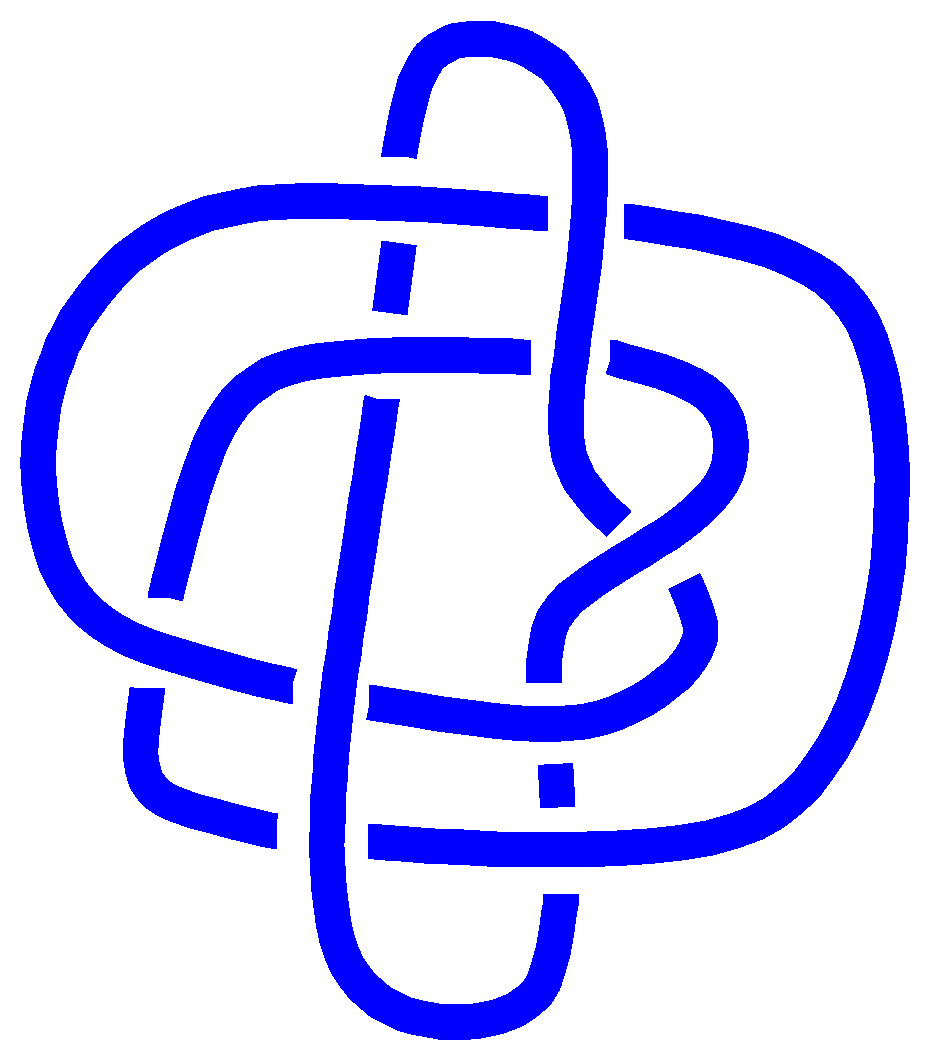
\includegraphics[scale=0.1]{../images/Perko1.pdf} &
   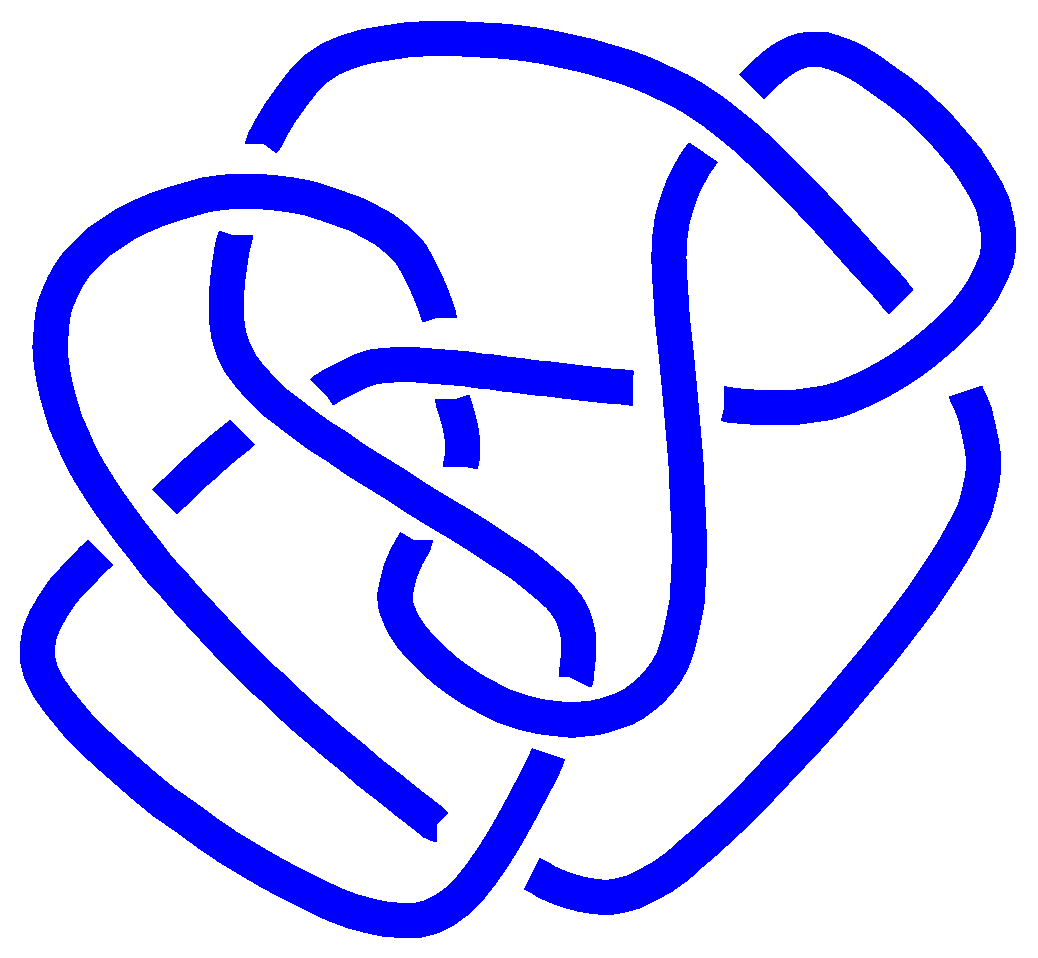
\includegraphics[scale=0.1]{../images/Perko2.pdf} &
   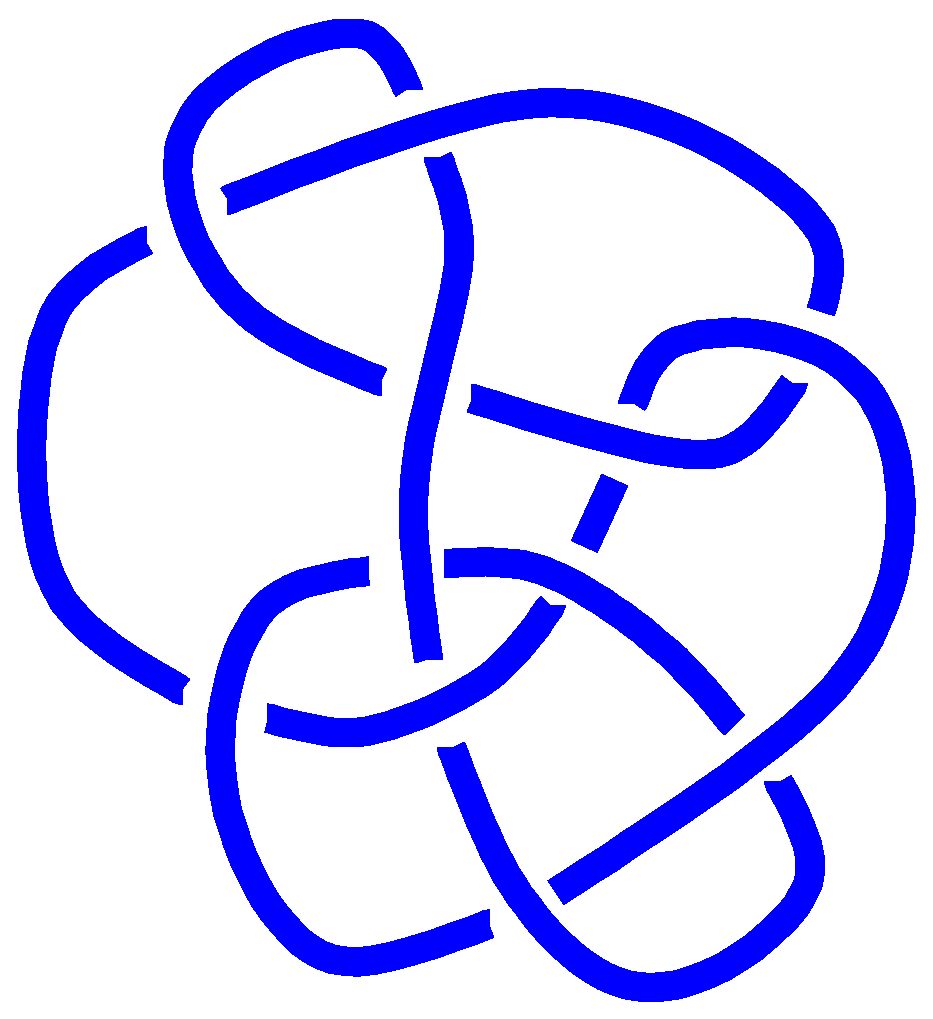
\includegraphics[scale=0.1]{../images/Conway.pdf} &
   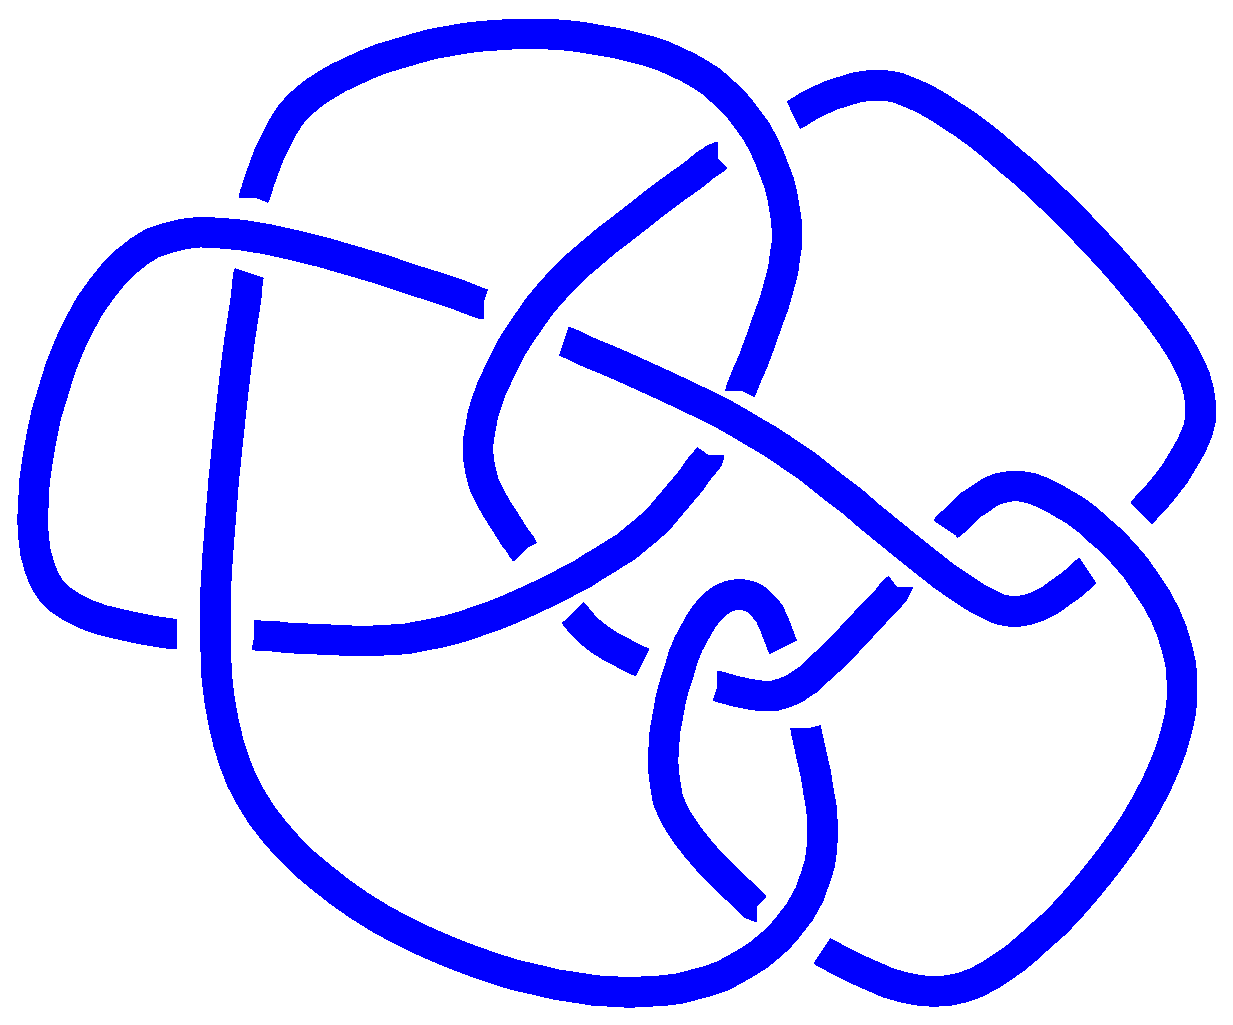
\includegraphics[scale=0.1]{../images/Kinoshita.pdf} \\
   $K_0$ & $K_1$ & $K_2$ & $K_3$ 
  \end{tabular}
 \end{center}
 It can be shown that 
 \begin{align*}
  f(K_0) = f(K_1) &= A^{-12} + A^{-24} - A^{-28} + A^{-32} - A^{-36} + A^{-40} - A^{-44} \\
  f(K_2) = f(K_3) &= -A^{16} + 2A^{12}-2A^{8} + 2A^3 + A^{-8}-2A^{-12} + 2A^{-16}-2A^{-20} + A^{-24}.
 \end{align*}
 What can you deduce from this?
\end{exercise}
\begin{solution}
 We deduce that 
 \begin{itemize}
  \item $K_0$ is not equivalent to $K_2$ 
  \item $K_0$ is not equivalent to $K_3$ 
  \item $K_1$ is not equivalent to $K_2$ 
  \item $K_1$ is not equivalent to $K_3$.
 \end{itemize}
 We do not have enough information to decide whether $K_0$ is
 equivalent to $K_1$, or whether $K_2$ is equivalent to $K_3$.  (In
 fact, $K_0$ and $K_1$ are equivalent, but $K_2$ and $K_3$ are not;
 however, the methods needed to prove that are beyond the scope of this
 course.) 
 \vspace{3ex}
\end{solution}
\vspace{-3ex}
\begin{exercise}
 Write down all states $S$ of the underlying universes
 for the following link diagrams $D$. For each state calculate
 $\langle D|S\rangle$ and $|S|$. Hence write down the unnormalized
 bracket $\un{D}$. \vspace{-6ex}
 \begin{center}
  \begin{tikzpicture}
   \begin{scope}
    \draw[black] ( 0,-1) node {$D_1$};
    \draw[black] ( 3,-1) node {$D_2$};
    \draw[black] ( 6,-1) node {$D_3$};
    \draw[black] ( 9,-1) node {$D_4$};
    \draw[white] (0,-2.3) -- (1,-2.3);
   \end{scope}
   \begin{scope}[scale=0.35]
    \node (a) at ( 0.00, 1.00) {};
    \node (b) at ( 0.00,-1.00) {};
    \draw[blue] (a) .. controls (a.4 south east) and (b.4 north east) ..
                (b.center) .. controls (b.16 south west) and (a.16 north west) .. (a);
    \draw[red]  (a.center) .. controls (a.4 south west) and (b.4 north west) ..
                (b) .. controls (b.16 south east) and (a.16 north east) .. (a.center);
   \end{scope}
   \begin{scope}[xshift=3cm,xscale=0.5,yscale=0.9]
    \node (a) at (0,0) {};
    \draw (a.center) .. controls (a.16 north east) and (a.16 south east) ..
          (a) .. controls (a.16 north west) and (a.16 south west) .. (a.center);
   \end{scope}
   \begin{scope}[xshift=6cm,xscale=1,yscale=1.3]
    \node (a) at (0,0) {};
    \node (b) at (1,0) {};
    \draw (a.center) .. controls (a.4 north east) and (b.4 north west) ..
          (b)        .. controls (b.8 south east) and (b.8 north east) ..
          (b.center) .. controls (b.4 south west) and (a.4 south east) .. 
          (a)        .. controls (a.8 north west) and (a.8 south west) .. (a.center);
   \end{scope}
   \begin{scope}[xshift=9cm,scale=0.35]
    \node (a) at ( 0.00, 1.00) {};
    \node (b) at ( 0.00,-1.00) {};
    \draw[blue] (a.center) .. controls (a.4 south east) and (b.4 north east) ..
                (b.center) .. controls (b.16 south west) and (a.16 north west) .. (a.center);
    \draw[red]  (a) .. controls (a.4 south west) and (b.4 north west) ..
                (b) .. controls (b.16 south east) and (a.16 north east) .. (a);
   \end{scope}
  \end{tikzpicture}
 \end{center} 
 \vspace{-8ex}
\end{exercise}
\begin{solution}
 The states for the $D_1$ are as follows
 \begin{center}
  \begin{tikzpicture}[scale=0.5]
   \draw[thin,black] (-5,-2.5) rectangle (-3,2.5);
   \draw[black] (-4,0) node {\huge $S$};
   \draw[thin,black] (-5,-7.5) rectangle (-3,-2.5);
   \draw[black] (-4,-5) node {\huge $D/S$};
   \draw[black] (-4,-8.25) node {\huge $|S|$};
   \draw[thin,black] (-5,-9) rectangle (-3,-7.5); 
   \draw[thin,black] (-3,-9) rectangle ( 3,-7.5); 
   \draw[thin,black] ( 3,-9) rectangle ( 9,-7.5); 
   \draw[thin,black] ( 9,-9) rectangle (15,-7.5); 
   \draw[thin,black] (15,-9) rectangle (21,-7.5); 
   \draw[black] ( 0,-8.25) node {\huge $2$};
   \draw[black] ( 6,-8.25) node {\huge $1$};
   \draw[black] (12,-8.25) node {\huge $1$};
   \draw[black] (18,-8.25) node {\huge $2$};
   \draw[thin,black] (-5,-10.5) rectangle (-3,-9); 
   \draw[thin,black] (-3,-10.5) rectangle ( 3,-9); 
   \draw[thin,black] ( 3,-10.5) rectangle ( 9,-9); 
   \draw[thin,black] ( 9,-10.5) rectangle (15,-9); 
   \draw[thin,black] (15,-10.5) rectangle (21,-9); 
   \draw[black] (-4,-9.75) node {\huge $\ip{D|S}$};
   \draw[black] ( 0,-9.75) node {\huge $A^2$};
   \draw[black] ( 6,-9.75) node {\huge $AB$};
   \draw[black] (12,-9.75) node {\huge $AB$};
   \draw[black] (18,-9.75) node {\huge $B^2$};
   \begin{scope}
    \node (a) at ( 0.00, 1.00) {};
    \node (b) at ( 0.00,-1.00) {};
    \draw[blue] (a) .. controls (a.4 south east) and (b.4 north east) ..
                (b.center) .. controls (b.16 south west) and (a.16 north west) .. (a);
    \draw[blue]  (a.center) .. controls (a.4 south west) and (b.4 north west) ..
                (b) .. controls (b.16 south east) and (a.16 north east) .. (a.center);
    \draw[orange] (0, 0.6) -- (0, 1.4);
    \draw[orange] (0,-0.6) -- (0,-1.4);
    \draw[black] (0, 1.9) node {\huge $A$};
    \draw[black] (0,-1.9) node {\huge $A$};
    \draw[thin,black] (-3,-2.5) rectangle (3,2.5);
   \end{scope}
   \begin{scope}[xshift=6cm]
    \node (a) at ( 0.00, 1.00) {};
    \node (b) at ( 0.00,-1.00) {};
    \draw[blue] (a) .. controls (a.4 south east) and (b.4 north east) ..
                (b.center) .. controls (b.16 south west) and (a.16 north west) .. (a);
    \draw[blue]  (a.center) .. controls (a.4 south west) and (b.4 north west) ..
                (b) .. controls (b.16 south east) and (a.16 north east) .. (a.center);
    \draw[orange] (0, 0.6) -- (0, 1.4);
    \draw[orange] (-0.4,-1) -- (0.4,-1);
    \draw[black] (0, 1.9) node {\huge $A$};
    \draw[black] (-0.8,-1) node {\huge $B$};
    \draw[thin,black] (-3,-2.5) rectangle (3,2.5);
   \end{scope}
   \begin{scope}[xshift=12cm]
    \node (a) at ( 0.00, 1.00) {};
    \node (b) at ( 0.00,-1.00) {};
    \draw[blue] (a) .. controls (a.4 south east) and (b.4 north east) ..
                (b.center) .. controls (b.16 south west) and (a.16 north west) .. (a);
    \draw[blue]  (a.center) .. controls (a.4 south west) and (b.4 north west) ..
                (b) .. controls (b.16 south east) and (a.16 north east) .. (a.center);
    \draw[orange] (-0.4,1) -- (0.4,1);
    \draw[orange] (0,-0.6) -- (0,-1.4);
    \draw[black] (0,-1.9) node {\huge $A$};
    \draw[black] (-0.8,1) node {\huge $B$};
    \draw[thin,black] (-3,-2.5) rectangle (3,2.5);
   \end{scope}
   \begin{scope}[xshift=18cm]
    \node (a) at ( 0.00, 1.00) {};
    \node (b) at ( 0.00,-1.00) {};
    \draw[blue] (a) .. controls (a.4 south east) and (b.4 north east) ..
                (b.center) .. controls (b.16 south west) and (a.16 north west) .. (a);
    \draw[blue]  (a.center) .. controls (a.4 south west) and (b.4 north west) ..
                (b) .. controls (b.16 south east) and (a.16 north east) .. (a.center);
    \draw[orange] (-0.4,1) -- (0.4,1);
    \draw[orange] (-0.4,-1) -- (0.4,-1);
    \draw[black] (-0.8, 1) node {\huge $B$};
    \draw[black] (-0.8,-1) node {\huge $B$};
    \draw[thin,black] (-3,-2.5) rectangle (3,2.5);
   \end{scope}
   \begin{scope}[yshift=-5cm]
    \node (a) at ( 0.00, 1.00) {};
    \node (b) at ( 0.00,-1.00) {};
    \draw[blue] (a) .. controls (a.4 south east) and (b.4 north east) ..
                (b.center) .. controls (b.16 south west) and (a.16 north west) .. (a);
    \draw[blue]  (a.center) .. controls (a.4 south west) and (b.4 north west) ..
                (b) .. controls (b.16 south east) and (a.16 north east) .. (a.center);
    \fill[white] (-0.35, 0.65) rectangle + (0.7, 0.7);
    \fill[white] (-0.35,-0.65) rectangle + (0.7,-0.7);
    \draw (-0.29, 0.65) -- (-0.29, 1.35);
    \draw ( 0.29, 0.65) -- ( 0.29, 1.35);
    \draw (-0.29,-0.65) -- (-0.29,-1.35);
    \draw ( 0.29,-0.65) -- ( 0.29,-1.35);
    \draw[thin,black] (-3,-2.5) rectangle (3,2.5);
   \end{scope}
   \begin{scope}[yshift=-5cm,xshift=6cm]
    \node (a) at ( 0.00, 1.00) {};
    \node (b) at ( 0.00,-1.00) {};
    \draw[blue] (a) .. controls (a.4 south east) and (b.4 north east) ..
                (b.center) .. controls (b.16 south west) and (a.16 north west) .. (a);
    \draw[blue]  (a.center) .. controls (a.4 south west) and (b.4 north west) ..
                (b) .. controls (b.16 south east) and (a.16 north east) .. (a.center);
    \fill[white] (-0.35, 0.65) rectangle + (0.7, 0.7);
    \fill[white] (-0.35,-0.65) rectangle + (0.7,-0.7);
    \draw (-0.29, 0.65) -- (-0.29, 1.35);
    \draw ( 0.29, 0.65) -- ( 0.29, 1.35);
    \draw (-0.29,-0.65) -- ( 0.29,-0.65);
    \draw (-0.29,-1.30) -- ( 0.29,-1.30);
    \draw[thin,black] (-3,-2.5) rectangle (3,2.5);
   \end{scope}
   \begin{scope}[yshift=-5cm,xshift=12cm]
    \node (a) at ( 0.00, 1.00) {};
    \node (b) at ( 0.00,-1.00) {};
    \draw[blue] (a) .. controls (a.4 south east) and (b.4 north east) ..
                (b.center) .. controls (b.16 south west) and (a.16 north west) .. (a);
    \draw[blue]  (a.center) .. controls (a.4 south west) and (b.4 north west) ..
                (b) .. controls (b.16 south east) and (a.16 north east) .. (a.center);
    \fill[white] (-0.35, 0.65) rectangle + (0.7, 0.7);
    \fill[white] (-0.35,-0.65) rectangle + (0.7,-0.7);
    \draw (-0.29, 0.65) -- ( 0.29, 0.65);
    \draw (-0.29, 1.30) -- ( 0.29, 1.30);
    \draw (-0.29,-0.65) -- (-0.29,-1.35);
    \draw ( 0.29,-0.65) -- ( 0.29,-1.35);
    \draw[thin,black] (-3,-2.5) rectangle (3,2.5);
   \end{scope}
   \begin{scope}[yshift=-5cm,xshift=18cm]
    \node (a) at ( 0.00, 1.00) {};
    \node (b) at ( 0.00,-1.00) {};
    \draw[blue] (a) .. controls (a.4 south east) and (b.4 north east) ..
                (b.center) .. controls (b.16 south west) and (a.16 north west) .. (a);
    \draw[blue]  (a.center) .. controls (a.4 south west) and (b.4 north west) ..
                (b) .. controls (b.16 south east) and (a.16 north east) .. (a.center);
    \fill[white] (-0.35, 0.65) rectangle + (0.7, 0.7);
    \fill[white] (-0.35,-0.65) rectangle + (0.7,-0.7);
    \draw (-0.29, 0.65) -- ( 0.29, 0.65);
    \draw (-0.29, 1.30) -- ( 0.29, 1.30);
    \draw (-0.29,-0.65) -- ( 0.29,-0.65);
    \draw (-0.29,-1.30) -- ( 0.29,-1.30);
    \draw[thin,black] (-3,-2.5) rectangle (3,2.5);
   \end{scope}
  \end{tikzpicture}
 \end{center}   
 From this we get 
 \[ \un{D_1} = A^2C + 2AB + B^2C. \]
 For $D_2$, the states are as follows:
 \begin{center}
  \begin{tikzpicture}
   \draw[thin,black] (-2.5, 1) rectangle (-1.5,-1);
   \draw[thin,black] (-1.5, 1) rectangle ( 1.5,-1);
   \draw[thin,black] ( 1.5, 1) rectangle ( 4.5,-1);
   \draw[thin,black] (-2.5,-1) rectangle (-1.5,-2);
   \draw[thin,black] (-1.5,-1) rectangle ( 1.5,-2);
   \draw[thin,black] ( 1.5,-1) rectangle ( 4.5,-2);
   \draw[thin,black] (-2.5,-2) rectangle (-1.5,-3);
   \draw[thin,black] (-1.5,-2) rectangle ( 1.5,-3);
   \draw[thin,black] ( 1.5,-2) rectangle ( 4.5,-3);
   \draw[black] (-2, 0.0) node {$S$};
   \draw[black] (-2,-1.5) node {$|S|$};
   \draw[black] (-2,-2.5) node {$\ip{D|S}$};
   \draw[black] ( 0,-1.5) node {$2$};
   \draw[black] ( 3,-1.5) node {$1$};
   \draw[black] ( 0,-2.5) node {$A$};
   \draw[black] ( 3,-2.5) node {$B$};
   \begin{scope}[xscale=0.5,yscale=0.9]
     \node (a) at (0,0) {};
     \draw (a.center) .. controls (a.16 north east) and (a.16 south east) ..
           (a) .. controls (a.16 north west) and (a.16 south west) .. (a.center);
     \draw[orange] (0,-0.4) -- (0,0.4);
   \end{scope}
   \begin{scope}[xshift=3cm,xscale=0.5,yscale=0.9]
     \node (a) at (0,0) {};
     \draw (a.center) .. controls (a.16 north east) and (a.16 south east) ..
           (a) .. controls (a.16 north west) and (a.16 south west) .. (a.center);
     \draw[orange] (-0.6,0) -- (0.6,0);
   \end{scope}
  \end{tikzpicture}
 \end{center}
 This gives $\un{D_2}=AC+B$.  The other two diagrams can be analysed
 in a similar way, giving 
 \begin{align*}
  \un{D_3} &= A^2C^2 + 2ABC + B^2 \\
  \un{D_4} &= A^2 + 2ABC + B^2.
 \end{align*}
\end{solution}
\vspace{-4ex}
\begin{exercise}
 For each of the following diagrams write splitting markers for
 the ``all A'' state $S_A$ and the ``all B'' state $S_B$. Calculate
 $|S_A|$ and $|S_B|$. 
 \begin{center}
  \begin{tikzpicture}[scale=0.5]
   \begin{scope}
    \node (a) at (-0.50, 1.00) {};
    \node (b) at ( 0.50, 1.00) {};
    \node (c) at ( 0.00, 0.00) {};
    \node (d) at ( 0.00,-1.00) {};
    \draw (a) -- (b.center) 
     .. controls (b.8 east) and (d.8 south east) .. (d)
     .. controls (d.4 north west) and (c.4 south west) .. (c.center)
     .. controls (c.4 north east) and (b.4 south) .. (b)
     .. controls (b.4 north) and (a.4 north) .. (a.center)
     .. controls (a.4 south) and (c.4 north west) .. (c)
     .. controls (c.4 south east) and (d.4 north east) ..(d.center)
     .. controls (d.8 south west) and (a.8 west) .. (a); 
   \end{scope}
   \begin{scope}[xshift=6cm]
    \node (a) at (-2, 1) {};
    \node (b) at (-2, 0) {};
    \node (c) at (-2,-1) {};
    \node (d) at ( 0, 1) {};
    \node (e) at ( 0,-1) {};
    \node (f) at ( 2, 1) {};
    \node (g) at ( 2, 0) {};
    \node (h) at ( 2,-1) {};
    \draw
     (a.center) .. controls (a.4 south east) and (b.4 north east) ..
     (b)        .. controls (b.4 south west) and (c.4 north west) ..
     (c.center) .. controls (c.4 south east) and (e.4 south west) ..
     (e.center) .. controls (e.4 north east) and (d.4 south east) ..
     (d.center) .. controls (d.4 north west) and (a.4 north east) ..
     (a)        .. controls (a.4 south west) and (b.4 north west) ..
     (b.center) .. controls (b.4 south east) and (c.4 north east) ..
     (c)        .. controls (c.8 south west) and (-1,-1.8) ..
     (0,-1.8)   .. controls (1,-1.8) and (h.8 south east) ..
     (h)        .. controls (h.4 north west) and (g.4 south west) ..
     (g.center) .. controls (g.4 north east) and (f.4 south east) ..
     (f)        .. controls (f.4 north west) and (d.4 north east) ..
     (d)        .. controls (d.4 south west) and (e.4 north west) ..
     (e)        .. controls (e.4 south east) and (h.4 south west) ..
     (h.center) .. controls (h.4 north east) and (g.4 south east) ..
     (g)        .. controls (g.4 north west) and (f.4 south west) ..
     (f.center) .. controls (f.8 north east) and (1,1.8) ..
     (0, 1.8)   .. controls (-1,1.8) and (a.8 north west) .. (a.center);    
   \end{scope}
  \end{tikzpicture}
 \end{center}
\end{exercise}
\begin{solution}
 For the first diagram, we have $|S_A|=|S_B|=3$.  
 \begin{center}
  \begin{tikzpicture}
   \begin{scope}
    \node (a) at (-0.50, 1.00) {};
    \node (b) at ( 0.50, 1.00) {};
    \node (c) at ( 0.00, 0.00) {};
    \node (d) at ( 0.00,-1.00) {};
    \draw (a) -- (b.center) 
     .. controls (b.8 east) and (d.8 south east) .. (d)
     .. controls (d.4 north west) and (c.4 south west) .. (c.center)
     .. controls (c.4 north east) and (b.4 south) .. (b)
     .. controls (b.4 north) and (a.4 north) .. (a.center)
     .. controls (a.4 south) and (c.4 north west) .. (c)
     .. controls (c.4 south east) and (d.4 north east) ..(d.center)
     .. controls (d.8 south west) and (a.8 west) .. (a); 
    \draw[orange] (-0.8,1.3) -- (-0.2,0.7);
    \draw[orange] ( 0.8,1.3) -- ( 0.2,0.7);
    \draw[orange] (0,-0.4) -- (0,0.4);
    \draw[orange] (0,-1.4) -- (0,-0.6);
    \draw[black] (0,-2) node {$S_A$};
   \end{scope}
   \begin{scope}[xshift=4cm]
    \node (a) at (-0.50, 1.00) {};
    \node (b) at ( 0.50, 1.00) {};
    \node (c) at ( 0.00, 0.00) {};
    \node (d) at ( 0.00,-1.00) {};
    \draw (a) -- (b.center) 
     .. controls (b.8 east) and (d.8 south east) .. (d)
     .. controls (d.4 north west) and (c.4 south west) .. (c.center)
     .. controls (c.4 north east) and (b.4 south) .. (b)
     .. controls (b.4 north) and (a.4 north) .. (a.center)
     .. controls (a.4 south) and (c.4 north west) .. (c)
     .. controls (c.4 south east) and (d.4 north east) ..(d.center)
     .. controls (d.8 south west) and (a.8 west) .. (a); 
    \fill[white] (-0.7, 0.8) rectangle (-0.3, 1.2);
    \fill[white] ( 0.3, 0.8) rectangle ( 0.7, 1.2);
    \fill[white] (-0.2,-0.2) rectangle ( 0.2, 0.2);
    \fill[white] (-0.2,-1.2) rectangle ( 0.2,-0.8);
    \draw (-0.7, 1.0) -- (-0.5, 0.8);
    \draw (-0.5, 1.2) -- (-0.3, 1.0);
    \draw ( 0.7, 1.0) -- ( 0.5, 0.8);
    \draw ( 0.5, 1.2) -- ( 0.3, 1.0);
    \draw (-0.2, 0.2) -- (-0.2,-0.2);
    \draw ( 0.2, 0.2) -- ( 0.2,-0.2);
    \draw (-0.2,-0.8) -- (-0.2,-1.2);
    \draw ( 0.2,-1.2) -- ( 0.2,-0.8);
    \draw[black] (0,-2) node {$D/S_A$};
   \end{scope}
   \begin{scope}[xshift=9cm]
    \node (a) at (-0.50, 1.00) {};
    \node (b) at ( 0.50, 1.00) {};
    \node (c) at ( 0.00, 0.00) {};
    \node (d) at ( 0.00,-1.00) {};
    \draw (a) -- (b.center) 
     .. controls (b.8 east) and (d.8 south east) .. (d)
     .. controls (d.4 north west) and (c.4 south west) .. (c.center)
     .. controls (c.4 north east) and (b.4 south) .. (b)
     .. controls (b.4 north) and (a.4 north) .. (a.center)
     .. controls (a.4 south) and (c.4 north west) .. (c)
     .. controls (c.4 south east) and (d.4 north east) ..(d.center)
     .. controls (d.8 south west) and (a.8 west) .. (a); 
    \draw[orange] (-0.8,0.7) -- (-0.2,1.3);
    \draw[orange] ( 0.8,0.7) -- ( 0.2,1.3);
    \draw[orange] (-0.4, 0) -- (0.4, 0);
    \draw[orange] (-0.4,-1) -- (0.4,-1);
    \draw[black] (0,-2) node {$S_B$};
   \end{scope}
   \begin{scope}[xshift=13cm]
    \node (a) at (-0.50, 1.00) {};
    \node (b) at ( 0.50, 1.00) {};
    \node (c) at ( 0.00, 0.00) {};
    \node (d) at ( 0.00,-1.00) {};
    \draw (a) -- (b.center) 
     .. controls (b.8 east) and (d.8 south east) .. (d)
     .. controls (d.4 north west) and (c.4 south west) .. (c.center)
     .. controls (c.4 north east) and (b.4 south) .. (b)
     .. controls (b.4 north) and (a.4 north) .. (a.center)
     .. controls (a.4 south) and (c.4 north west) .. (c)
     .. controls (c.4 south east) and (d.4 north east) ..(d.center)
     .. controls (d.8 south west) and (a.8 west) .. (a); 
    \fill[white] (-0.7, 0.8) rectangle (-0.3, 1.2);
    \fill[white] ( 0.3, 0.8) rectangle ( 0.7, 1.2);
    \fill[white] (-0.2,-0.2) rectangle ( 0.2, 0.2);
    \fill[white] (-0.2,-1.2) rectangle ( 0.2,-0.8);
    \draw (-0.7, 1.0) -- (-0.5, 1.2);
    \draw (-0.3, 1.0) -- (-0.5, 0.8);
    \draw ( 0.7, 1.0) -- ( 0.5, 1.2);
    \draw ( 0.5, 0.8) -- ( 0.3, 1.0);
    \draw (-0.2, 0.2) -- ( 0.2, 0.2);
    \draw (-0.2,-0.2) -- ( 0.2,-0.2);
    \draw (-0.2,-0.8) -- ( 0.2,-0.8);
    \draw ( 0.2,-1.2) -- (-0.2,-1.2);
    \draw[black] (0,-2) node {$D/S_B$};
   \end{scope}
  \end{tikzpicture}
 \end{center}
 For the second diagram, these pictures show that $|S_A|=3$.
 \begin{center}
  \begin{tikzpicture}
   \begin{scope}
    \node (a) at (-2, 1) {};
    \node (b) at (-2, 0) {};
    \node (c) at (-2,-1) {};
    \node (d) at ( 0, 1) {};
    \node (e) at ( 0,-1) {};
    \node (f) at ( 2, 1) {};
    \node (g) at ( 2, 0) {};
    \node (h) at ( 2,-1) {};
    \draw
     (a.center) .. controls (a.4 south east) and (b.4 north east) ..
     (b)        .. controls (b.4 south west) and (c.4 north west) ..
     (c.center) .. controls (c.4 south east) and (e.4 south west) ..
     (e.center) .. controls (e.4 north east) and (d.4 south east) ..
     (d.center) .. controls (d.4 north west) and (a.4 north east) ..
     (a)        .. controls (a.4 south west) and (b.4 north west) ..
     (b.center) .. controls (b.4 south east) and (c.4 north east) ..
     (c)        .. controls (c.8 south west) and (-1,-1.8) ..
     (0,-1.8)   .. controls (1,-1.8) and (h.8 south east) ..
     (h)        .. controls (h.4 north west) and (g.4 south west) ..
     (g.center) .. controls (g.4 north east) and (f.4 south east) ..
     (f)        .. controls (f.4 north west) and (d.4 north east) ..
     (d)        .. controls (d.4 south west) and (e.4 north west) ..
     (e)        .. controls (e.4 south east) and (h.4 south west) ..
     (h.center) .. controls (h.4 north east) and (g.4 south east) ..
     (g)        .. controls (g.4 north west) and (f.4 south west) ..
     (f.center) .. controls (f.8 north east) and (1,1.8) ..
     (0, 1.8)   .. controls (-1,1.8) and (a.8 north west) .. (a.center);    
    \draw[orange] (-2.4,-1.0) -- (-1.6,-1.0);
    \draw[orange] (-2.4, 0.0) -- (-1.6, 0.0);
    \draw[orange] (-2.4, 1.0) -- (-1.6, 1.0);
    \draw[orange] (-0.4, 1.0) -- ( 0.4, 1.0);
    \draw[orange] ( 0.0,-1.4) -- ( 0.0,-0.6);
    \draw[orange] ( 2.0,-1.4) -- ( 2.0,-0.6);
    \draw[orange] ( 2.0,-0.4) -- ( 2.0, 0.4);
    \draw[orange] ( 2.0, 0.6) -- ( 2.0, 1.4);
    \draw[black] (0,-2.4) node {$S_A$};
   \end{scope}
   \begin{scope}[xshift=7cm]
    \node (a) at (-2, 1) {};
    \node (b) at (-2, 0) {};
    \node (c) at (-2,-1) {};
    \node (d) at ( 0, 1) {};
    \node (e) at ( 0,-1) {};
    \node (f) at ( 2, 1) {};
    \node (g) at ( 2, 0) {};
    \node (h) at ( 2,-1) {};
    \draw
     (a.center) .. controls (a.4 south east) and (b.4 north east) ..
     (b)        .. controls (b.4 south west) and (c.4 north west) ..
     (c.center) .. controls (c.4 south east) and (e.4 south west) ..
     (e.center) .. controls (e.4 north east) and (d.4 south east) ..
     (d.center) .. controls (d.4 north west) and (a.4 north east) ..
     (a)        .. controls (a.4 south west) and (b.4 north west) ..
     (b.center) .. controls (b.4 south east) and (c.4 north east) ..
     (c)        .. controls (c.8 south west) and (-1,-1.8) ..
     (0,-1.8)   .. controls (1,-1.8) and (h.8 south east) ..
     (h)        .. controls (h.4 north west) and (g.4 south west) ..
     (g.center) .. controls (g.4 north east) and (f.4 south east) ..
     (f)        .. controls (f.4 north west) and (d.4 north east) ..
     (d)        .. controls (d.4 south west) and (e.4 north west) ..
     (e)        .. controls (e.4 south east) and (h.4 south west) ..
     (h.center) .. controls (h.4 north east) and (g.4 south east) ..
     (g)        .. controls (g.4 north west) and (f.4 south west) ..
     (f.center) .. controls (f.8 north east) and (1,1.8) ..
     (0, 1.8)   .. controls (-1,1.8) and (a.8 north west) .. (a.center);    
    \fill[white] (-2.3, 0.7) rectangle + (0.6,0.6);
    \fill[white] (-2.3,-0.3) rectangle + (0.6,0.6);
    \fill[white] (-2.3,-1.3) rectangle + (0.6,0.6);
    \fill[white] (-0.3, 0.7) rectangle + (0.6,0.6);
    \fill[white] (-0.3,-1.3) rectangle + (0.6,0.6);
    \fill[white] ( 1.7, 0.7) rectangle + (0.6,0.6);
    \fill[white] ( 1.7,-0.3) rectangle + (0.6,0.6);
    \fill[white] ( 1.7,-1.3) rectangle + (0.6,0.6);
    \draw (-2.30, 1.30) -- (-1.70, 1.27);
    \draw (-2.30, 0.70) -- (-1.70, 0.70);
    \draw (-2.30, 0.30) -- (-1.70, 0.30);
    \draw (-2.30,-0.30) -- (-1.70,-0.30);
    \draw (-2.30,-0.70) -- (-1.70,-0.70);
    \draw (-2.30,-1.30) -- (-1.70,-1.27);
    \draw (-0.30, 1.25) -- ( 0.30, 1.25);
    \draw (-0.27, 0.75) -- ( 0.27, 0.75);
    \draw (-0.27,-0.70) -- (-0.27,-1.30);
    \draw ( 0.27,-0.70) -- ( 0.27,-1.30);
    \draw ( 1.70, 1.25) -- ( 1.70, 0.75);
    \draw ( 1.70, 0.25) -- ( 1.70,-0.25);
    \draw ( 1.70,-0.75) -- ( 1.70,-1.25); 
    \draw ( 2.30, 1.25) -- ( 2.30, 0.75);
    \draw ( 2.30, 0.25) -- ( 2.30,-0.25);
    \draw ( 2.30,-0.75) -- ( 2.30,-1.25); 
    \draw[black] (0,-2.4) node {$D/S_A$};
   \end{scope}
  \end{tikzpicture}
 \end{center}
 A very similar picture also shows that $|S_B|=3$.
\end{solution}

\begin{exercise}
 For the standard diagram of the negative Hopf link, calculate the
 Kauffman bracket and hence the Jones polynomial.  (You calculated the
 unnormalized bracket in Sheet 3 Exercise 4.)  Check that your answer
 agrees with the answer obtained in lectures using the skein relation.
\end{exercise}

\begin{exercise}
 Consider the following four diagrams related to the figure eight knot:
 \begin{center}
  \begin{tikzpicture}
   \begin{scope}
    \node (a) at (-0.50,-1.00) {};
    \node (b) at ( 0.50,-1.00) {};
    \node (c) at ( 0.00, 0.00) {};
    \node (d) at ( 0.00, 1.00) {};
    \draw (a) -- (b.center) 
     .. controls (b.8 east) and (d.8 north east) .. (d)
     .. controls (d.4 south west) and (c.4 north west) .. (c.center)
     .. controls (c.4 south east) and (b.4 north) .. (b)
     .. controls (b.4 south) and (a.4 south) .. (a.center)
     .. controls (a.4 north) and (c.4 south west) .. (c)
     .. controls (c.4 north east) and (d.4 south east) ..(d.center)
     .. controls (d.8 north west) and (a.8 west) .. (a); 
    \draw[->] ( 0.1,-1.44) -- +( 0.01,0); 
    \draw[->] ( 0.0,-1.00) -- +(-0.01,0); 
    \draw[->] ( 0.3, 0.47) -- +( 0,-0.01); 
    \draw[->] (-0.3, 0.53) -- +( 0, 0.01); 
    \draw[black] (0,-2) node {$D$};
   \end{scope}
   \begin{scope}[xshift=4cm]
    \node (a) at (-0.50,-1.00) {};
    \node (b) at ( 0.50,-1.00) {};
    \node (c) at ( 0.00, 0.00) {};
    \node (d) at ( 0.00, 1.00) {};
    \draw (a) -- (b.center) 
     .. controls (b.8 east) and (d.8 north east) .. (d)
     .. controls (d.4 south west) and (c.4 north west) .. (c.center)
     .. controls (c.4 south east) and (b.4 north) .. (b)
     .. controls (b.4 south) and (a.4 south) .. (a.center)
     .. controls (a.4 north) and (c.4 south west) .. (c)
     .. controls (c.4 north east) and (d.4 south east) ..(d.center)
     .. controls (d.8 north west) and (a.8 west) .. (a); 
    \draw[->] ( 0.0,-1.44) -- +(-0.01,0); 
    \draw[->] ( 0.1,-1.00) -- +( 0.01,0); 
    \draw[->] ( 0.3, 0.50) -- +( 0, 0.01); 
    \draw[->] (-0.3, 0.47) -- +( 0,-0.01); 
    \draw[black] (0,-2) node {$D^*$};
   \end{scope}
   \begin{scope}[xshift=8cm]
    \node (a) at (-0.50,-1.00) {};
    \node (b) at ( 0.50,-1.00) {};
    \node (c) at ( 0.00, 0.00) {};
    \node (d) at ( 0.00, 1.00) {};
    \draw (a.center) -- (b) 
     .. controls (b.8 east) and (d.8 north east) .. (d.center)
     .. controls (d.4 south west) and (c.4 north west) .. (c)
     .. controls (c.4 south east) and (b.4 north) .. (b.center)
     .. controls (b.4 south) and (a.4 south) .. (a)
     .. controls (a.4 north) and (c.4 south west) .. (c.center)
     .. controls (c.4 north east) and (d.4 south east) ..(d)
     .. controls (d.8 north west) and (a.8 west) .. (a.center); 
    \draw[->] ( 0.1,-1.44) -- +( 0.01,0); 
    \draw[->] ( 0.0,-1.00) -- +(-0.01,0); 
    \draw[->] ( 0.3, 0.47) -- +( 0,-0.01); 
    \draw[->] (-0.3, 0.53) -- +( 0, 0.01); 
    \draw[black] (0,-2) node {$\ov{D}$};
   \end{scope}
   \begin{scope}[xshift=12cm]
    \node (a) at (-0.50,-1.00) {};
    \node (b) at ( 0.50,-1.00) {};
    \node (c) at ( 0.00, 0.00) {};
    \node (d) at ( 0.00, 1.00) {};
    \draw (a.center) -- (b) 
     .. controls (b.8 east) and (d.8 north east) .. (d.center)
     .. controls (d.4 south west) and (c.4 north west) .. (c)
     .. controls (c.4 south east) and (b.4 north) .. (b.center)
     .. controls (b.4 south) and (a.4 south) .. (a)
     .. controls (a.4 north) and (c.4 south west) .. (c.center)
     .. controls (c.4 north east) and (d.4 south east) ..(d)
     .. controls (d.8 north west) and (a.8 west) .. (a.center); 
    \draw[->] ( 0.0,-1.44) -- +(-0.01,0); 
    \draw[->] ( 0.1,-1.00) -- +( 0.01,0); 
    \draw[->] ( 0.3, 0.50) -- +( 0, 0.01); 
    \draw[->] (-0.3, 0.47) -- +( 0,-0.01); 
    \draw[black] (0,-2) node {$\ov{D}^*$};
   \end{scope}
  \end{tikzpicture}
 \end{center}
 Show that they are all R-equivalent, so the figure 8 is both
 reversible and amphicheiral.  (It is not too hard to give an
 R-equivalence $D\sim D^*$ by imagining what would happen if you
 rotated $D$ around a vertical line.  The same approach gives
 $\ov{D}\sim\ov{D}^*$.  However, it is harder to show that
 $D\sim\ov{D}$, and you will probably need to experiment with string.)

 Now calculate $f(D)$ using the Kauffman bracket, and check that you
 get the same answer as the one obtained in the lecture using the
 skein relation.
\end{exercise}

\begin{exercise}
 The following two knots respectively have Jones polynomials
 $-A^{32}+A^{20}+A^{12}$ and $A^{12}-A^8+A^4-1+A^{-4}-A^{-8}+A^{-12}.$
 \[ 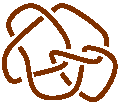
\includegraphics[scale=1.3]{../images/knot8_19.pdf}
    \hspace{4em}
    
\includegraphics[scale=1.3]{../images/knot9_42.pdf}
 \]
 What can you deduce about the symmetry properties of these knots?
\end{exercise}

\begin{exercise}
 Let $f_1(D)$ be the number obtained by substituting $A=1$
 in $f(D)$.
 \begin{itemize}
  \item[(a)] Deduce from Exercise~4 on Problem Sheet~1 that any link
   can be converted to an unlink by switching crossings.
  \item[(b)] By thinking about the skein relation, show that $f_1(D)$ only
   depends on the underlying universe of $D$, not on the overcrossings
   or undercrossings.  
  \item[(c)] Now deduce that $f_1(D)=2^{c-1}$, where $c$ is the number of
   components in $D$.  Thus, we can find the number of components in
   $D$ by inspecting the Jones polynomial. 
  \item[(d)] Deduce that the sum of coefficients of the Jones polynomial
   of a \emph{knot} is always equal to 1.
  \item[(e)] (Optional) What is the sum of coefficients of the
   \emph{derivative} of the Jones polynomial of a knot?
 \end{itemize} 
\end{exercise}

\begin{exercise}
 For each of the following sets, decide whether is is a closed
 surface, a surface with boundary, or not a surface. 

 \begin{align*}
  X_0 &= \{(x,y,z)\in\R^3\st x^2+y^2+z^2\leq 1\} \\
  X_1 &= \{(w,x,y,z)\in\R^4\st w^2+x^2=y^2+z^2=1\} \\
  X_2 &= \{(x,y,z)\in\R^3\st x,y,z\geq 0,\; x+y+z = 1\} \\
  X_3 &= \{(x,y)\in\R^2\st x^2+y^2<1\} \\
  X_4 &= \{(x,y,z)\in\R^3\st x^2+y^2+z^2\leq 1,\; xyz=0\} \\
  X_5 &= \{(w,x,y,z)\in\R^4\st w+z=0,\;w^2+x^2+y^2+z^2=1\}.
 \end{align*}
\end{exercise}
\begin{solution}
 \begin{itemize}
  \item The space $X_0$ is not a surface, because it is solid.  The point
   $(0,0,0)\in X_0$ has an open neighbourhood homeomorphic to the
   $3$-dimensional open ball, but has no neighbourhood homeomorphic to
   the $2$-dimensional open disc.
  \item The space $X_1$ is a surface, and in fact is homeomorphic to a torus.
   Indeed, we can define 
   \[ f(s,t)=(\cos(2\pi s),\sin(2\pi s),\cos(2\pi t),\sin(2\pi t)), \]
   and then $X_1$ is precisely the image of the map $f$.  Given any
   point $a\in X_1$, we can choose $(s,t)$ such that $a=f(s,t)$, then
   we can define a map $g$ from the open unit disc to $X_1$ by
   $g(x,y)=f(s+x,t+y)$.  This identifies the open unit disc with a
   neighbourhood of $a$ in $X_1$.  Alternatively, we can say that
   every point in $X_1$ has the form $f(s,t)$ for some point $(s,t)$
   in the unit square, and this point is unique except that
   $f(s,0)=f(s,1)$ and $f(0,t)=f(1,t)$.  In other words, the left and
   right edges of the square have the same image in $X_1$, as do the
   top and bottom edges.  This is precisely the gluing pattern for the
   torus.
  \item The space $X_2$ is just a triangle, with vertices $(1,0,0)$,
   $(0,1,0)$ and $(0,0,1)$.  Any triangle is homeomorphic to a closed
   disc which is a surface with boundary, so $X_2$ is a also surface
   with boundary.
  \item The space $X_3$ is not compact, because it contains the
   sequence of points $(1-1/n,0)$, which converge to the point
   $(1,0)$, which is not in $X_3$.  Thus, $X_3$ is not a surface
   according to our definitions.  (However, every point has a full
   disc neighbourhood, so it is a surface according to some other
   people's definitions.)
  \item Note that the condition $xyz=0$ means that $x=0$ or $y=0$ or
   $z=0$.  This means that the space $X_4$ can be thought of as the
   union of three closed unit discs, one in the $xy$-plane, one in the
   $xz$-plane and one in the $yz$-plane.  If a point lies on the
   intersection of two of these discs, then it will not have a disc of
   half-disc neighbourhood in $X_4$.  Thus, $X_4$ is not a surface.
  \item For $X_5$, note that the condition $w+z=0$ gives $w=-z$ and so
   $w^2=z^2$.  Given this, the condition $w^2+x^2+y^2+z^2=1$ becomes
   $x^2+y^2+(\sqrt{2}z)^2=1$.  Thus, the map
   $(w,x,y,z)\mapsto(x,y,\sqrt{2}z)$ gives a homeomorphism from $X_5$
   to $S^2$, showing that $X_5$ is a surface.
 \end{itemize}
\end{solution}

\begin{exercise}
 Consider the space
 \[ X = \{(x,y,z)\in\R^3\st x^2+y^2+z^2=1,
           -0.9 \leq x,y,z\leq 0.9\}.
 \]
 This is homeomorphic to $D^{\# n}$ for some $n$.  What is $n$?
\end{exercise}
\begin{solution}
 The condition $x^2+y^2+z^2=1$ describes a sphere.  The equation
 $x=0.9$ describes a plane, which passes through the sphere close to
 the point $(1,0,0)$.  The inequality $x\leq 0.9$ cuts off a small
 disc around that point, leaving a hole in the sphere.  Similarly, the
 remaining inequalities $-0.9\leq x,y,z\leq 0.9$ cut out holes near
 the points $(-1,0,0)$, $(0,1,0)$, $(0,-1,0)$, $(0,0,1)$ and
 $(0,0,-1)$.  That gives six holes in total.  We showed in the notes
 that $Z\# D$ is the same as $Z$ with a disc removed.  Thus, we have
 $X\simeq S^2\#D^{\# 6}$.  On the other hand, $S^2\# Z$ is the same as
 $Z$, so $X\simeq D^{\# 6}$.  In other words, $n=6$.
\end{solution}

\begin{exercise}
 The space below is homeomorphic to $T^{\# n}$ for some $n$ (where $T$
 is the torus).  What is $n$?
 \[ 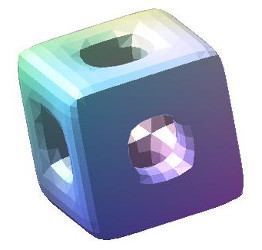
\includegraphics[scale=0.6]{../images/holycube.jpg} \]
\end{exercise}
\begin{solution}
 We can flatten out and distort the surface as shown in the following
 series of pictures.
 \[ 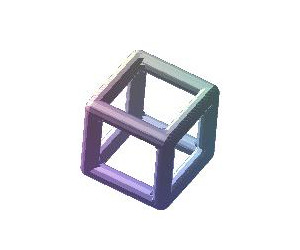
\includegraphics[scale=0.5]{../images/holycube_flatten0.jpg}
    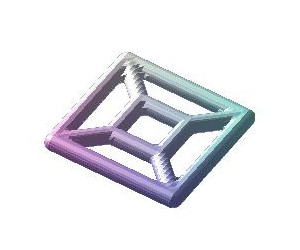
\includegraphics[scale=0.5]{../images/holycube_flatten1.jpg}
    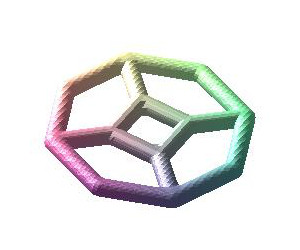
\includegraphics[scale=0.5]{../images/holycube_flatten2.jpg}
 \]
 \[ 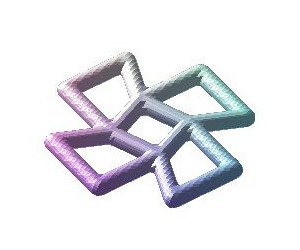
\includegraphics[scale=0.5]{../images/holycube_flatten3.jpg}
    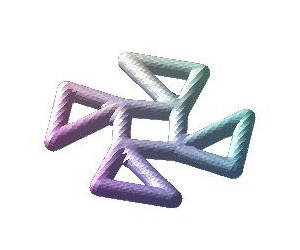
\includegraphics[scale=0.5]{../images/holycube_flatten4.jpg}
 \]
 The last picture is the connected sum of a (square) torus in the
 middle with four (triangular) tori around the outside.  Thus, we have
 $X\simeq T^{\# 5}$ and so $n=5$.
\end{solution}

\begin{exercise}\label{ex-octahedron}
 Here is a picture of an octahedron, with vertices labelled $1$ to
 $6$.  We write $26$ for the edge joining vertices $2$ and $6$, and
 $135$ for the triangle with vertices $1$, $3$ and $5$ and so on.
 \begin{center}
  \begin{tikzpicture}[scale=1.5]
   \draw[black,dashed] (0.513,0.245) -- (-1.41,0.0891);
   \draw[black,dashed] (0.513,0.245) -- (0,1.48);
   \draw[black,dashed] (0.513,0.245) -- (1.41,-0.0891);
   \draw[black,dashed] (0.513,0.245) -- (0,-1.48);
   \draw[black] (-1.41,0.0891) -- (0,1.48);
   \draw[black] (-1.41,0.0891) -- (-0.513,-0.245);
   \draw[black] (-1.41,0.0891) -- (0,-1.48);
   \draw[black] (0,1.48) -- (-0.513,-0.245);
   \draw[black] (0,1.48) -- (1.41,-0.0891);
   \draw[black] (-0.513,-0.245) -- (1.41,-0.0891);
   \draw[black] (-0.513,-0.245) -- (0,-1.48);
   \draw[black] (1.41,-0.0891) -- (0,-1.48);
   \fill[black] (0.513,0.245) circle(0.03);
   \fill[black] (-1.41,0.0891) circle(0.03);
   \fill[black] (0,1.48) circle(0.03);
   \fill[black] (-0.513,-0.245) circle(0.03);
   \fill[black] (1.41,-0.0891) circle(0.03);
   \fill[black] (0,-1.48) circle(0.03);
   \draw[black] (0.636,0.314) node {$\scriptstyle{4}$};
   \draw[black] (-1.69,0.107) node {$\scriptstyle{5}$};
   \draw[black] (0,1.77) node {$\scriptstyle{3}$};
   \draw[black] (-0.616,-0.324) node {$\scriptstyle{1}$};
   \draw[black] (1.69,-0.107) node {$\scriptstyle{2}$};
   \draw[black] (0,-1.77) node {$\scriptstyle{6}$};
  \end{tikzpicture}
 \end{center}
 The eight triangles give a closed linear surface triangulation of the
 surface of the octahedron, as defined in Definition~\ref{defn-triangulation}.
 If we just consider the top four triangles, then they give a linear
 surface triangulation with boundary of the top half of the
 octahedron.  Explain carefully why these statements are true, with
 examples.
\end{exercise}
\begin{solution}
 For a closed linear surface triangulation, the first condition is
 that the intersection any pair of distinct triangles should be empty,
 a common vertex or a common edge.  For example:
 \begin{itemize}
  \item The triangles $123$ and $456$ have empty intersection.
  \item The triangles $123$ and $246$ meet only at point $2$, which
   is a vertex of both triangles.
  \item The intersection of triangles $123$ and $126$ is the line
   segment $12$, which is an edge of both of the tiangles.
 \end{itemize}
 One can check that all other pairs of triangles also follow one of
 the above patterns.

 The second condition is that each edge should be an edge of precisely
 two triangles.  For example:
 \begin{itemize}
  \item The edge $12$ is an edge of the triangles $123$ and $126$ (and
   no others).
  \item The edge $13$ is an edge of the triangles $123$ and $135$ (and
   no others).
  \item The edge $56$ is an edge of the triangles $156$ and $456$ (and
   no others).
 \end{itemize}
 One can check all twelve edges in the same way.

 The last condition concerns the pattern of triangles containing any
 given vertex.  For example, the triangles containing point $1$ can be
 listed as follows:
 \[ T_1 = 123 \qquad
    T_2 = 135 \qquad
    T_3 = 156 \qquad
    T_4 = 126.
 \]
 Here 
 \begin{itemize}
  \item $T_1$ shares the edge $13$ with $T_2$;
  \item $T_2$ shares the edge $15$ with $T_3$;
  \item $T_3$ shares the edge $16$ with $T_4$;
  \item $T_4$ shares the edge $11$ with $T_1$;
  \item there are no other shared edges.
 \end{itemize}
 This verifies the required condition for vertex $1$, and one can do
 the same for all other vertices.
\end{solution}

\begin{exercise}
 Using Exercise~\ref{ex-octahedron} or otherwise, prove that the
 sphere $S^2$ is homeomorphic to a PL closed surface.
\end{exercise}
\begin{solution}
 If we place our octahedron $X$ with the origin at the centre, then we
 can define a homeomorphism $f\:X\to S^2$ by $f(u)=u/\|u\|$.
\end{solution}

\begin{exercise}
 For each of the following words $W_k$, describe the surface
 $\Sg(W_k)$.  In particular, you should state whether $\Sg(W_k)$ is
 orientable, whether it has a boundary, and which of the surfaces in
 the notes it is homeomorphic to.
 \[ W_1 = ba\db\,\cb\,dc\bb\,\ab \qquad
    W_2 = ba\db\,\cb\,dcba \qquad
    W_3 = abb\ab \qquad
    W_4 = abac \qquad
    W_5 = abc\cb\,\ab\,\bb \qquad
    W_6 = abc\cb a\bb.
 \]
\end{exercise}
\begin{solution}
 \begin{itemize}
  \item In $W_2$, every letter occurs once barred and once unbarred,
   so the corresponding surface is closed and orientable.  The word
   can be rotated to give $\db\cb dc\bb\ab ba$, which
   can be relabelled as $uv\ub\vb wx\wb\xb$.  This is two copies of the
   torus word $T$, and we have seen that $TV\sim T\#V$ for any $V$, so
   $W_1\sim T\# T$.  Thus, $\Sg(W_1)$ is the connected sum of two
   tori.  In particular, it is closed and orientable.
  \item In $W_2$ every letter occurs twice, but both copies of $a$ are
   unbarred.  This means that the surface is closed but not
   orientable.  We have surface moves as follows:
   \[ W_2 = b[a\db\,\cb\,dc]ba 
          \sim bb\cb\db cd(\ab a)
          \sim bb\cb\db cd 
          \cong PT \sim P\# T.
   \]
   Thus, $\Sg(W_2)$ is the connected sum of a torus and a projective
   plane.
  \item The moves $W_3=abb|\ab\sim (\ab a)bb\sim bb\cong P$ show that
   $\Sg(W_3)$ is a projective plane, which is again closed and not
   orientable.
  \item $W_4$ is the standard word for the M\"obius strip; it is
   neither closed nor orientable.
  \item We can cancel $c\,\cb$ to see that $W_5\sim T$, so $\Sg(W_5)$
   is a torus, which is closed and orientable.
  \item We have word moves as follows:
   \[ W_6 = ab(c\cb)a\bb \sim a[b]a\bb \sim aa\bb\bb \cong PP
       \sim P\# P,
   \]
   so $\Sg(W_6)$ is the connected sum of two projective planes.
 \end{itemize}
\end{solution}

\begin{exercise}
 How many different surfaces (up to homeomorphism) can be constructed
 as $\Sg(W)$ with $W$ a word of length $4$?
\end{exercise}
\begin{solution}
 I claim that the possibilities are as follows:
 \begin{align*}
  D     &\simeq \Sg(abcd) \\
  D\# D &\simeq \Sg(abc\bb) \\
  P\# D &\simeq \Sg(aabc) \\
  P\# P &\simeq \Sg(aabb) \\
  P     &\simeq \Sg(aab\bb) \\ 
  T     &\simeq \Sg(ab\ab\bb) \\
  S     &\simeq \Sg(a\ab b\bb).
 \end{align*}
 To justify this, we first need to check that $\Sg(abcd)$ really is
 homeomorphic to $D$, and similarly for the other equations above.
 This is true by merger moves for $D$, by definition for $D\#D$ and
 $T$, and by cancellation for $P$ and $S$.  For the remaining cases
 $P\#D$ and $P\# P$, we need the general fact that $P\# V\sim PV$ for
 all $V$.

 Next, we need to check that any word $W$ of length four is equivalent
 to one of those listed above.  
 \begin{itemize}
  \item If $W$ has four unmatched letters, then after relabelling it is
   the same as $abcd$ and so gives $D$.
  \item Suppose next that $W$ has two unmatched letters, and one
   letter that occurs twice, once barred and once unbarred.  If the
   matched letters are adjacent then they can be cancelled and we get
   $D$ again.  This also works (after rotation) if one copy is at the
   beginning and the other copy is at the end.  In the only remaining
   case, we can relabel and rotate if necessary to get $abc\bb$, which
   gives $D\# D$.
  \item Suppose next that $W$ has two unmatched letters, and one
   letter that occurs twice with the same barring.  After a crosscap
   move, we can assume that the matched letters are adjacent.  After
   rotation, we can assume that they occur at the beginning.  After
   relabelling, we now have $aabc$.  After merging $bc$ this becomes
   $aab=PD\sim P\# D$.
  \item Now suppose we have two matched pairs.  If one or the other
   pair is nonorientable, then we can perform a crosscap move to make
   that pair adjacent, and then rotate it to the beginning.  This will
   give us either $aabb=PP\sim P\# P$ or $aab\bb\sim aa=P$.  
  \item Suppose instead that we have two matched pairs, both
   orientable.  If either pair is adjacent then we can cancel it, and
   then the other pair will become adjacent, so we can cancel it as
   well, giving $S$.
  \item Finally, suppose we have two matched orientable pairs, neither
   of which is adjacent.  After relabelling this must just be
   $ab\ab\bb$, which gives $T$.
 \end{itemize}
\end{solution}

\begin{exercise}
 Show by example that if $U$ and $V$ are non-closed surface words,
 then $UV$ need not be equivalent to $U\# V$.
\end{exercise}
\begin{solution}
 The simplest possible example will do: we just take $U=x$ and $V=y$,
 so $UV\sim U$ by a merger move, and so $\Sg(UV)$ is a disk.  However,
 $\Sg(U\# V)$ is a connected sum of two discs, which is homeomorphic
 to a cylinder.
\end{solution}

\begin{exercise}
 Show (directly from the definition of word equivalence) that an
 orientable word can never be equivalent to a non-orientable word, and
 a closed word can never be equivalent to a non-closed word.
\end{exercise}
\begin{solution}
 It will be sufficient to consider a single word move.  We first
 consider orientability.  For the purposes of this discussion, a
 ``precisely repeated letter'' means a letter which occurs twice
 barred or twice unbarred.
 \begin{itemize}
  \item As $UV$ and $VU$ have exactly the same letters in a different
   order, we see that $UV$ has a precisely repeated letter if and only
   if $VU$ does.  Thus, a rotation does not affect orientability.
   Neither does an inner rotation, by the same argument.
  \item Now consider a cancellation $Ux\xb V\to UV$.  If $UV$ has a
   precisely repeated letter, then that must also be present in
   $Ux\xb V$.  Conversely, suppose that $Ux\xb V$ contains a precisely
   repeated letter.  That letter cannot be $x$, because $x$ is only
   allowed to occur twice, so we still have the precisely repeated
   letter in $UV$.  Thus, cancellation does not affect orientability.
  \item In a crosscap move $TxUxV\to Txx\ov{U}V$, both of the words
   are visibly nonorientable, because of the repeated $x$; we do not
   need to worry about what might be present in $T$, $U$ or $V$.
  \item In a merger move $UxyV\to UxV$, the letters $x$ and $y$ are
   assumed not to be repeated.  From this it is clear that $UxyV$ has
   a precisely repeated letter if and only if $UxV$ does.
  \item It is also clear from the definitions that relabelling does
   not affect orientability.
 \end{itemize}

 Similar arguments work for closedness.
 \begin{itemize}
  \item As $UV$ and $VU$ have exactly the same letters in a different
   order, we see that $UV$ has an unmatched letter if and only
   if $VU$ does.  Thus, a rotation does not affect closedness.
   Neither does an inner rotation, by the same argument.
  \item Essentially the same argument works for a crosscap move.  That
   kind of move will add or subtract some bars as well as changing the
   order of the letters, but that does not affect the presence or
   absence of unmatched letters.
  \item Now consider a cancellation $Ux\xb V\to UV$.  This just
   removes a matched pair, so $UV$ has the same unmatched letters as
   $Ux\xb V$ (if any).
  \item In a merger move $UxyV\to UxV$, it is clear by assumption that
   both of the words are non-closed; we do not need to worry about
   what might be present in $U$ or $V$. 
  \item It is also clear from the definitions that relabelling does
   not affect closedness.
 \end{itemize}
\end{solution}

\begin{exercise}\leavevmode
 \begin{itemize}
  \item[(a)] Show that $a_1a_2U\ab_1\ab_2V\sim a_1a_2\ab_1\ab_2VU$.
  \item[(b)] Now put 
   \[ W_n = a_1a_2a_3\dotsb a_n\ab_1\ab_2\ab_3\dotsb \ab_n. \]
   Prove that $W_{2m}\sim W_{2m+1}\sim T^{\# m}$ for all $m\geq 0$.
  \item[(c)] Give similar results for the words 
   \begin{align*}
    U_n &= a_1a_2a_3\dotsb a_n a_1a_2a_3\dotsb a_n \\
    V_n &= a_1a_2a_3\dotsb a_n a_n \dotsb a_3a_2a_1.
   \end{align*}
 \end{itemize}
\end{exercise}
\begin{solution}
 \begin{itemize}
  \item[(a)] 
   $a_1a_2(U|\ab_1)\ab_2V\sim
    a_1a_2\ab_1(U|\ab_2V)\sim
    a_1a_2\ab_1\ab_2VU$.
   \item[(b)] The word $W_0$ is empty, and the word $W_1=a_1\ab_1$
    cancels down to the empty word, so $W_0\sim W_1\sim T^{\# 0}$.  
    Now suppose that $n\geq 2$.  Put $U=a_3\dotsb a_n$ and
    $V=\ab_3\dotsb\ab_n$, so $W_n=a_1a_2 U\ab_1\ab_2 V$.  By part~(a)
    we have $W_n\sim a_1a_2\ab_1\ab_2 VU=TVU\sim T\#VU$.  However,
    if we relabel $a_{i+2}$ as $\ab_i$ (and $\ab_{i+2}$ as $a_i$),
    then $VU$ becomes $W_{n-2}$.  We therefore see that
    $W_n\sim T\# W_{n-2}$.  It now follows easily by induction that
    $W_{2m}\sim W_{2m+1}\sim T^{\# m}$ for all $m\geq 0$.
   \item[(c)] The case of $U_n$ is very simple: a single crosscap move
    gives 
    \[ U_n \sim a_1a_1 \ab_n\dotsb \ab_3\ab_2 a_2a_3\dotsb a_n, \]
    and then we can cancel repeatedly to get $U_n\sim a_1a_1\cong P$.

    On the other hand, a crosscap move on $V_n$ produces 
    \[ V_n \sim a_1a_1 \ab_2\ab_3\dotsb \ab_n\ab_n\dotsb\ab_3\ab_2. \]
    The first pair of letters is a relabelled $P$, and the rest is a
    relabelled $V_{n-1}$, so $V_n\sim PV_{n-1}\sim P\# V_{n-1}$.  It
    is also clear that $V_0=S$ and $V_1=P$, so it follows inductively
    that $V_n\sim P^{\# n}$ for all $n$.
 \end{itemize}
\end{solution}

\begin{exercise}
 Draw several different surfaces that are all homeomorphic to the
 connected sum of three tori.
\end{exercise}
\begin{solution}
 Here are some possibilities:
 \[ 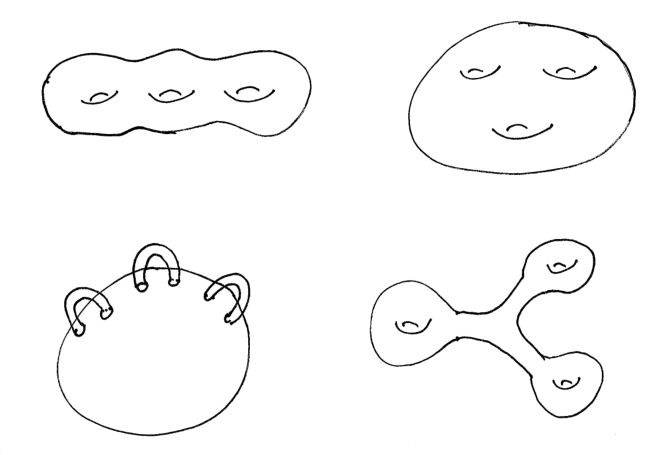
\includegraphics[scale=0.7]{../images/genus3_various.png} \]
\end{solution}

\begin{exercise}
 For each of the following surfaces, write down a corresponding word.
 Try to make it as short as possible.
 \begin{itemize}
  \item[(a)] A torus with two discs removed.
  \item[(b)] The connected sum of three tori.
  \item[(c)] The connected sum of a Klein bottle and a sphere.
  \item[(d)] A dodecahedron with two opposite faces removed.
 \end{itemize}
\end{exercise}
\begin{solution}
 \begin{itemize}
  \item[(a)] Removing a disc is the same as taking the connected sum
   with $D$.  Thus, the obvious answer is 
   \[ T\#(D\#D) = (ab\ab\,\bb)\#(def\db) = ab\ab\,\bb cdef\db\,\cb. \]
   However, this can be shortened slightly, because we know that
   $T\#U\sim TU$ for any $U$.  We can thus use the word
   \[ T(D\#D)  = ab\ab\bb def\db \]
   instead.
  \item[(b)] The obvious answer is just 
   \[ TTT = ab\ab\,\bb cd\cb\,\db\, ef\eb\,\fb. \]
  \item[(c)] Taking the connected sum with the sphere does not change
   anything, so we just want the standard Klein bottle word, which is
   $xy\xb y$.
  \item[(d)] The dodecahedron is just a sphere, and removing one face
   just leaves a disc.  To remove another hole, we just take the
   connected sum with a disc.  Thus, the word we want is just
   $D\# D=xyz\yb$.  Alternatively, one can see geometrically that
   removing two opposite faces leaves a surface which is homeomorphic
   to a cylinder, and the standard word for a cylinder is $xy\xb z$.
   This is equivalent by rotation and relabelling to the word
   $D\# D=xyz\yb$. 
 \end{itemize}
\end{solution}

\begin{exercise}
 Suppose that $U$, $V$ and $W$ are surface words, and that
 $U\# V\sim U\# W$.  Give an example to show that $V$ need not be
 equivalent to $W$.  Investigate this question in more detail, and
 formulate a clear and concise proposition about when we can or cannot
 conclude that $V\sim W$.
\end{exercise}
\begin{solution}
 First, take $U=P$ and $V=T$ and $W=P\# P$.  By
 Proposition~\ref{prop-PPP}, we have $U\# V\sim U\# W$.  However, $V$
 is orientable and $W$ is not, so $V$ and $W$ are not equivalent.  

 We have seen that any word is equivalent to $T^{\# i}\# D^{\# j}$
 or $P^{\#(i+1)}\#D^{\# j}$ (for some $i,j\geq 0$), and none of these
 words are equivalent to each other.  Connected sums are as follows: 
 \begin{align*}
  (T^{\# i}\# D^{\# j})\# (T^{\# n}\# D^{\# m}) 
   &\sim T^{\#(i+n)} \# D^{\#(j+m)} \\
  (T^{\# i}\# D^{\# j})\# (P^{\#(n+1)}\# D^{\# m}) 
   &\sim P^{\#(2i+n+1)} \# D^{\#(j+m)} \\
  (P^{\#(i+1)}\# D^{\# j})\# (T^{\# n}\# D^{\# m}) 
   &\sim P^{\#(i+2n+1)} \# D^{\#(j+m)} \\
  (P^{\#(i+1)}\# D^{\# j})\# (P^{\#(n+1)}\# D^{\# m}) 
   &\sim P^{\#(i+n+2)} \# D^{\#(j+m)}.
 \end{align*}
 From this table, we can deduce the following:
 \begin{proposition*}
  Suppose that $U$, $V$ and $W$ are surface words, and that
  $V\not\sim W$ but $U\# V\sim U\# W$.  Then $U$ must be
  nonorientable, and there must exist $i,j\geq 0$ such that either 
  \begin{itemize}
   \item[(a)] $V\sim T^{\#(i+1)}\# D^{\# j}$ and 
              $W\sim P^{\#(2i+2)}\# D^{\# j}$; or
   \item[(b)] $V\sim P^{\#(2i+2)}\# D^{\# j}$ and
              $W\sim T^{\#(i+1)}\# D^{\# j}$.
  \end{itemize}
 \end{proposition*}
\end{solution}

\end{document}
